\documentclass[12pt,a4paper]{article}

\usepackage{fontspec}
\usepackage[russian]{babel}
\usepackage{amsmath, amssymb}
\usepackage{geometry}
\usepackage{graphicx}
\usepackage{booktabs}
\usepackage{array}
\usepackage{float}
\usepackage{caption}
\usepackage{hyperref}
\usepackage{listings}
\usepackage{xcolor}

\setmainfont{Times New Roman}
\setsansfont{Arial}
\setmonofont{Menlo}

\geometry{margin=2cm}
\setlength{\parindent}{1.25cm}
\setlength{\parskip}{0.35em}

\lstset{
    basicstyle=\ttfamily\small,
    breaklines=true,
    frame=single,
    columns=fullflexible,
    keepspaces=true,
    extendedchars=true
}

\begin{document}

\begin{titlepage}
    \begin{center}
        Федеральное государственное автономное образовательное учреждение\\
        высшего образования\\
        <<Национальный исследовательский университет ИТМО>>

        \vspace*{0.28\textheight}

        {\Large \textbf{Отчёт}}\\
        {\large \textbf{По лабораторной работе №4}}\\
        {\large по дисциплине <<Вычислительная математика>>}\\
        {\large \textbf{Вариант: 4}}
    \end{center}

    \vfill

    \begin{flushright}
        Студент:\\
        Красноштанова Юлия Николаевна\\
        Группа Р3216\\
        Преподаватель:\\
        Наумова Надежда Александровна
    \end{flushright}

    \vfill

    \begin{center}
        г. Санкт-Петербург 2026
    \end{center}
\end{titlepage}

\section*{Цель работы}
Найти функцию, являющуюся наилучшим приближением заданной табличной функции по методу наименьших квадратов.

\section*{Задание}
\begin{enumerate}
    \item Предусмотреть ввод исходных данных из файла или с клавиатуры; таблица $y=f(x)$ должна содержать от 8 до 12 точек.
    \item Реализовать метод наименьших квадратов, исследуя линейную, полиномиальные 2-й и 3-й степени, экспоненциальную, логарифмическую и степенную функции.
    \item Вывести коэффициенты аппроксимирующих функций, среднеквадратичное отклонение и массивы значений $x_i$, $y_i$, $\varphi(x_i)$, $\varepsilon_i$.
    \item Для линейной зависимости вычислить коэффициент корреляции Пирсона.
    \item Вычислить коэффициент детерминации и вывести сообщение в зависимости от полученного значения $R^2$.
    \item Отобразить наилучшую аппроксимирующую функцию.
    \item Построить графики полученных эмпирических функций на всем исследуемом интервале с запасом.
    \item Протестировать программу при различных наборах данных, в том числе некорректных.
\end{enumerate}

\section*{Рабочие формулы}
Пусть задана таблица из $n$ точек $(x_i;y_i)$, $i=1,\ldots,n$. Мерой отклонения аппроксимирующей функции $\varphi(x)$ от табличных значений служит сумма квадратов отклонений:
\[
    S=\sum_{i=1}^{n}\varepsilon_i^2=\sum_{i=1}^{n}\bigl[\varphi(x_i)-y_i\bigr]^2 \to \min .
\]
Параметры функции $\varphi$ находятся из условия минимума $S$, то есть приравниванием к нулю частных производных $S$ по этим параметрам.

\subsection*{Линейная аппроксимация}
Для модели $\varphi(x)=ax+b$ условие минимума дает систему
\[
    \begin{cases}
        a\,S_{XX}+b\,S_X=S_{XY},\\
        a\,S_X+b\,n=S_Y,
    \end{cases}
    \qquad
    S_X=\sum x_i,\; S_{XX}=\sum x_i^2,\; S_Y=\sum y_i,\; S_{XY}=\sum x_iy_i .
\]
По правилу Крамера:
\[
    \Delta=S_{XX}\cdot n-S_X\cdot S_X,\qquad
    \Delta_1=S_{XY}\cdot n-S_X\cdot S_Y,\qquad
    \Delta_2=S_{XX}\cdot S_Y-S_X\cdot S_{XY},
\]
\[
    a=\frac{\Delta_1}{\Delta},\qquad b=\frac{\Delta_2}{\Delta}.
\]

\subsection*{Полиномиальная аппроксимация}
Для многочлена $\varphi(x)=a_0+a_1x+\ldots+a_mx^m$ система нормальных уравнений имеет вид
\[
    \sum_{j=0}^{m}a_j\sum_{i=1}^{n}x_i^{\,k+j}=\sum_{i=1}^{n}x_i^{\,k}y_i,\qquad k=0,1,\ldots,m,
\]
и решается методом Гаусса с выбором главного элемента по столбцу. В работе используются $m=2$ и $m=3$.

\subsection*{Аппроксимация линеаризуемыми функциями}
Степенная, экспоненциальная и логарифмическая зависимости приводятся к линейному виду $Y=A+BX$ заменой переменных, после чего применяется алгоритм линейной аппроксимации.

Степенная функция $\varphi(x)=ax^b$:
\[
    \ln\varphi(x)=\ln a+b\ln x,\qquad Y=\ln y,\; X=\ln x,\; A=\ln a,\; B=b
    \;\Longrightarrow\; a=e^{A},\; b=B.
\]
Экспоненциальная функция $\varphi(x)=ae^{bx}$:
\[
    \ln\varphi(x)=\ln a+bx,\qquad Y=\ln y,\; X=x,\; A=\ln a,\; B=b
    \;\Longrightarrow\; a=e^{A},\; b=B.
\]
Логарифмическая функция $\varphi(x)=a\ln x+b$ линейна по параметрам, достаточно замены $X=\ln x$, $Y=y$; найденные коэффициенты и есть искомые $a$ и $b$.

\begin{table}[H]
    \centering
    \caption{Замены переменных при линеаризации}
    \begin{tabular}{lcc}
        \toprule
        Вид функции & Табличный $X$ & Табличный $Y$\\
        \midrule
        $y=ax^b$ & $\ln x_i$ & $\ln y_i$\\
        $y=ae^{bx}$ & $x_i$ & $\ln y_i$\\
        $y=a\ln x+b$ & $\ln x_i$ & $y_i$\\
        \bottomrule
    \end{tabular}
\end{table}

Замены с $\ln x$ требуют $x>0$, замены с $\ln y$ требуют $y>0$. Если условие нарушено, соответствующая модель не может быть построена.

\subsection*{Оценка качества приближения}
Среднеквадратичное отклонение:
\[
    \delta=\sqrt{\frac{\sum_{i=1}^{n}\bigl(\varphi(x_i)-y_i\bigr)^2}{n}} .
\]
Наилучшим считается приближение с наименьшим $\delta$.

Коэффициент корреляции Пирсона для линейной зависимости:
\[
    r=\frac{\sum_{i=1}^{n}(x_i-\bar x)(y_i-\bar y)}
    {\sqrt{\sum_{i=1}^{n}(x_i-\bar x)^2\sum_{i=1}^{n}(y_i-\bar y)^2}},\qquad -1\le r\le 1 .
\]

Коэффициент детерминации:
\[
    R^2=1-\frac{\sum_{i=1}^{n}\bigl(y_i-\varphi_i\bigr)^2}{\sum_{i=1}^{n}\bigl(y_i-\bar\varphi\bigr)^2},
    \qquad \bar\varphi=\frac1n\sum_{i=1}^{n}\varphi_i .
\]
При $R^2\ge0{,}95$ точность аппроксимации высокая, при $0{,}75\le R^2<0{,}95$ -- удовлетворительная, при $0{,}5\le R^2<0{,}75$ -- слабая, при $R^2<0{,}5$ точность недостаточна и модель требует изменения.

\section*{Вычислительная часть}
Для варианта 4 задана функция
\[
    y=\frac{15x}{x^4+4},\qquad x\in[-4;\,0],\qquad h=0{,}4 .
\]
Таблица табулирования содержит 11 точек.

\begin{table}[H]
    \centering
    \footnotesize
    \setlength{\tabcolsep}{3pt}
    \caption{Таблица табулирования функции варианта 4}
    \begin{tabular}{l*{11}{c}}
        \toprule
        $x_i$ & $-4{,}0$ & $-3{,}6$ & $-3{,}2$ & $-2{,}8$ & $-2{,}4$ & $-2{,}0$ & $-1{,}6$ & $-1{,}2$ & $-0{,}8$ & $-0{,}4$ & $0{,}0$\\
        $y_i$ & $-0{,}2308$ & $-0{,}3140$ & $-0{,}4409$ & $-0{,}6416$ & $-0{,}9683$ & $-1{,}5000$ & $-2{,}2741$ & $-2{,}9636$ & $-2{,}7213$ & $-1{,}4905$ & $0{,}0000$\\
        \bottomrule
    \end{tabular}
\end{table}

\subsection*{Линейное приближение}
Вычислим суммы:
\[
    S_X=-22{,}0000,\qquad S_{XX}=61{,}6000,\qquad S_Y=-13{,}5451,\qquad S_{XY}=20{,}5530 .
\]
Система нормальных уравнений:
\[
    \begin{cases}
        61{,}6000\,a-22{,}0000\,b=20{,}5530,\\
        -22{,}0000\,a+11\,b=-13{,}5451 .
    \end{cases}
\]
Определители:
\[
\begin{aligned}
    \Delta &= 61{,}6000\cdot 11-(-22{,}0000)^2=677{,}6000-484{,}0000=193{,}6000,\\
    \Delta_1 &= 20{,}5530\cdot 11-(-22{,}0000)\cdot(-13{,}5451)=226{,}0830-297{,}9922=-71{,}9092,\\
    \Delta_2 &= 61{,}6000\cdot(-13{,}5451)-(-22{,}0000)\cdot 20{,}5530=-834{,}3782+452{,}1660=-382{,}2122 .
\end{aligned}
\]
Отсюда
\[
    a=\frac{-71{,}9092}{193{,}6000}=-0{,}371432,\qquad
    b=\frac{-382{,}2122}{193{,}6000}=-1{,}974236,
\]
\[
    P_1(x)=-0{,}371432\,x-1{,}974236 .
\]

\subsection*{Квадратичное приближение}
Вычислим суммы:
\[
\begin{aligned}
    &\sum x_i=-22{,}0000,\quad \sum x_i^2=61{,}6000,\quad \sum x_i^3=-193{,}6000,\quad \sum x_i^4=648{,}5248,\\
    &\sum y_i=-13{,}5451,\quad \sum x_iy_i=20{,}5530,\quad \sum x_i^2y_i=-40{,}9540 .
\end{aligned}
\]
Система нормальных уравнений:
\[
    \begin{cases}
        11\,a_0-22{,}0000\,a_1+61{,}6000\,a_2=-13{,}5451,\\
        -22{,}0000\,a_0+61{,}6000\,a_1-193{,}6000\,a_2=20{,}5530,\\
        61{,}6000\,a_0-193{,}6000\,a_1+648{,}5248\,a_2=-40{,}9540 .
    \end{cases}
\]
Решая систему методом Гаусса, получаем
\[
    a_0=-1{,}018187,\qquad a_1=1{,}221983,\qquad a_2=0{,}398354,
\]
\[
    P_2(x)=0{,}398354\,x^2+1{,}221983\,x-1{,}018187 .
\]

\subsection*{Проверка выбора моделей}
Подставим узлы $x_i$ в обе аппроксимирующие функции и найдем отклонения $\varepsilon_i=\varphi(x_i)-y_i$.

\begin{table}[H]
    \centering
    \small
    \caption{Значения аппроксимирующих функций и отклонения}
    \begin{tabular}{cccccc}
        \toprule
        $x_i$ & $y_i$ & $P_1(x_i)$ & $\varepsilon_i$ & $P_2(x_i)$ & $\varepsilon_i$\\
        \midrule
        $-4{,}0$ & $-0{,}2308$ & $-0{,}4885$ & $-0{,}2577$ & $0{,}4675$ & $0{,}6983$\\
        $-3{,}6$ & $-0{,}3140$ & $-0{,}6371$ & $-0{,}3231$ & $-0{,}2547$ & $0{,}0593$\\
        $-3{,}2$ & $-0{,}4409$ & $-0{,}7857$ & $-0{,}3448$ & $-0{,}8494$ & $-0{,}4085$\\
        $-2{,}8$ & $-0{,}6416$ & $-0{,}9342$ & $-0{,}2926$ & $-1{,}3166$ & $-0{,}6750$\\
        $-2{,}4$ & $-0{,}9683$ & $-1{,}0828$ & $-0{,}1145$ & $-1{,}6564$ & $-0{,}6881$\\
        $-2{,}0$ & $-1{,}5000$ & $-1{,}2314$ & $0{,}2686$ & $-1{,}8687$ & $-0{,}3687$\\
        $-1{,}6$ & $-2{,}2741$ & $-1{,}3799$ & $0{,}8942$ & $-1{,}9536$ & $0{,}3205$\\
        $-1{,}2$ & $-2{,}9636$ & $-1{,}5285$ & $1{,}4351$ & $-1{,}9109$ & $1{,}0527$\\
        $-0{,}8$ & $-2{,}7213$ & $-1{,}6771$ & $1{,}0442$ & $-1{,}7408$ & $0{,}9805$\\
        $-0{,}4$ & $-1{,}4905$ & $-1{,}8257$ & $-0{,}3352$ & $-1{,}4432$ & $0{,}0473$\\
        $0{,}0$ & $0{,}0000$ & $-1{,}9742$ & $-1{,}9742$ & $-1{,}0182$ & $-1{,}0182$\\
        \bottomrule
    \end{tabular}
\end{table}

Меры отклонения и среднеквадратичные отклонения:
\[
\begin{aligned}
    S_{P_1}&=\sum \varepsilon_i^2=8{,}420, &\qquad \delta_{P_1}&=\sqrt{\frac{8{,}420}{11}}=0{,}875,\\
    S_{P_2}&=\sum \varepsilon_i^2=4{,}934, &\qquad \delta_{P_2}&=\sqrt{\frac{4{,}934}{11}}=0{,}670 .
\end{aligned}
\]

\begin{table}[H]
    \centering
    \caption{Сравнение линейного и квадратичного приближений}
    \begin{tabular}{>{\raggedright\arraybackslash}p{5.1cm}ccc}
        \toprule
        Модель & Мера отклонения $S$ & $\delta$ & $R^2$\\
        \midrule
        Линейная, $P_1(x)=ax+b$ & 8,420 & 0,875 & 0,224\\
        Квадратичная, $P_2(x)=a_0+a_1x+a_2x^2$ & 4,934 & 0,670 & 0,545\\
        \bottomrule
    \end{tabular}
\end{table}

Коэффициент корреляции Пирсона для линейной модели равен $r=-0{,}4731$, что говорит о слабой линейной связи между $x$ и $y$ на данном интервале.

\textbf{Вывод по вычислительной части.} Наилучшим из двух рассмотренных приближений является квадратичное: у него меньше среднеквадратичное отклонение ($0{,}670$ против $0{,}875$) и выше коэффициент детерминации. Тем не менее и для него $R^2<0{,}75$, поэтому точность аппроксимации остается слабой -- заданная функция имеет на отрезке $[-4;0]$ минимум и точку перегиба, и многочлен второй степени не может воспроизвести такую форму.

\section*{Графики аппроксимирующих функций}
На рисунке приведены заданная функция, табличные точки и построенные линейное и квадратичное приближения.

\begin{figure}[H]
    \centering
    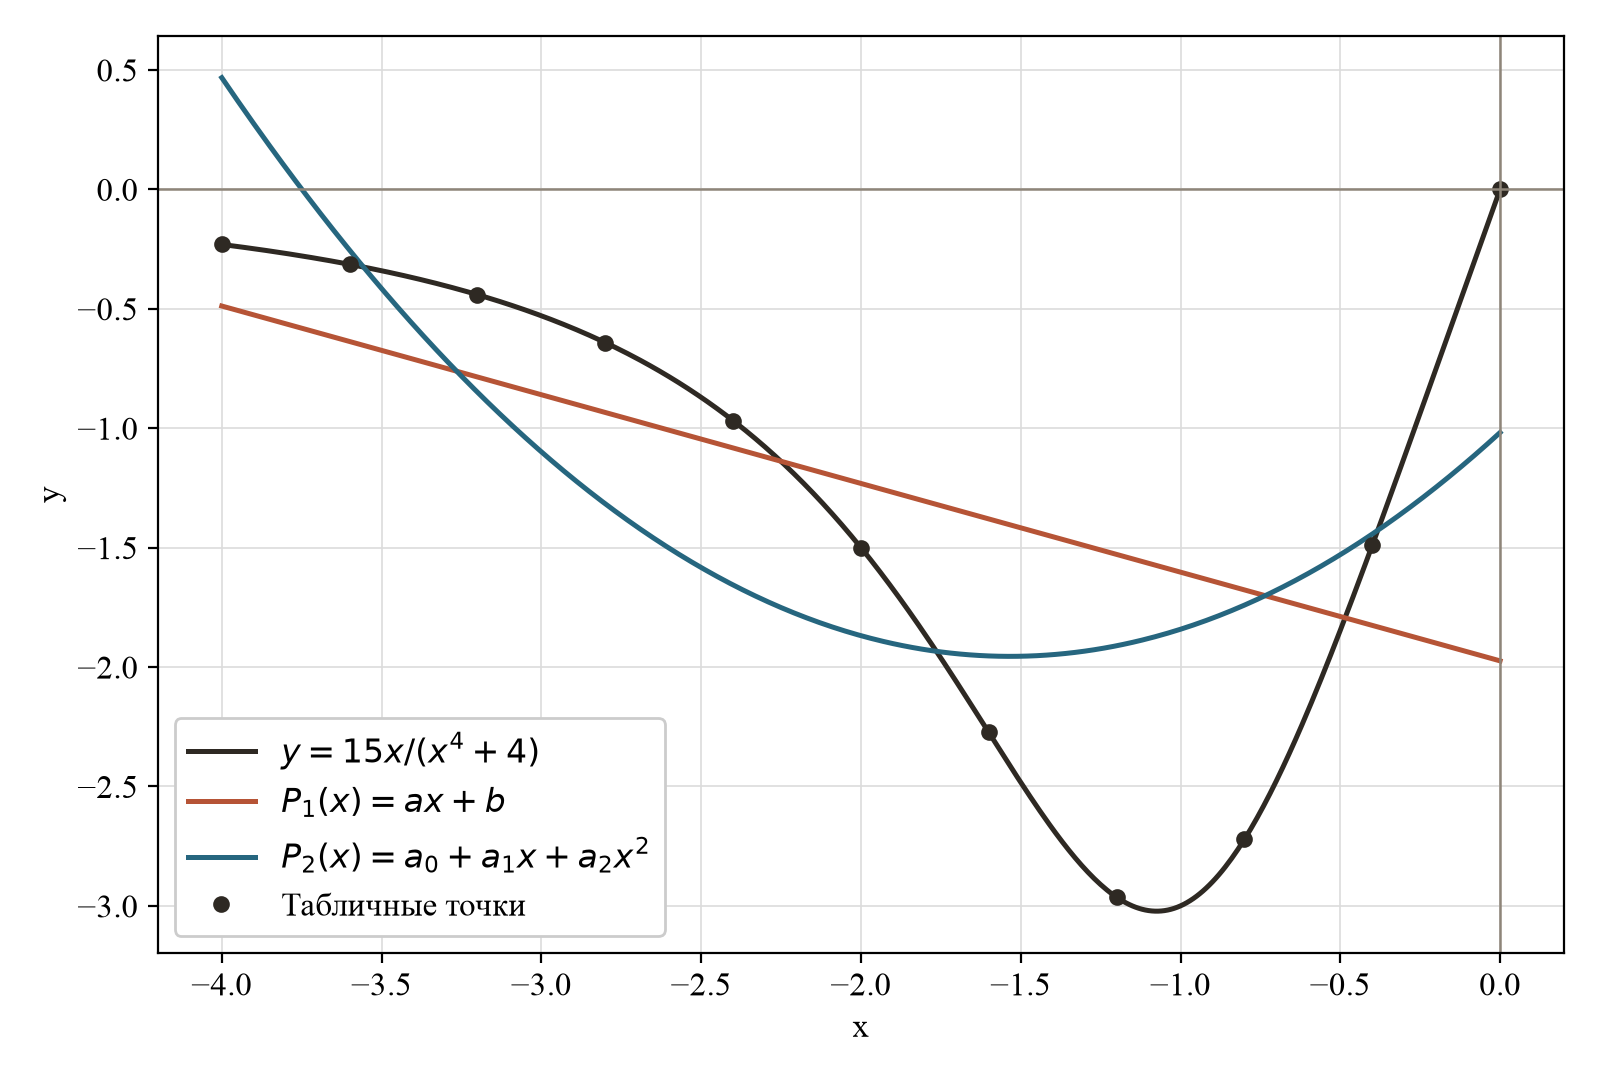
\includegraphics[width=\textwidth]{report_assets/computational_fit.png}
    \caption{Заданная функция и ее линейное и квадратичное приближения}
\end{figure}

Те же данные в программе: на графике включены только линейная и квадратичная модели.

\begin{figure}[H]
    \centering
    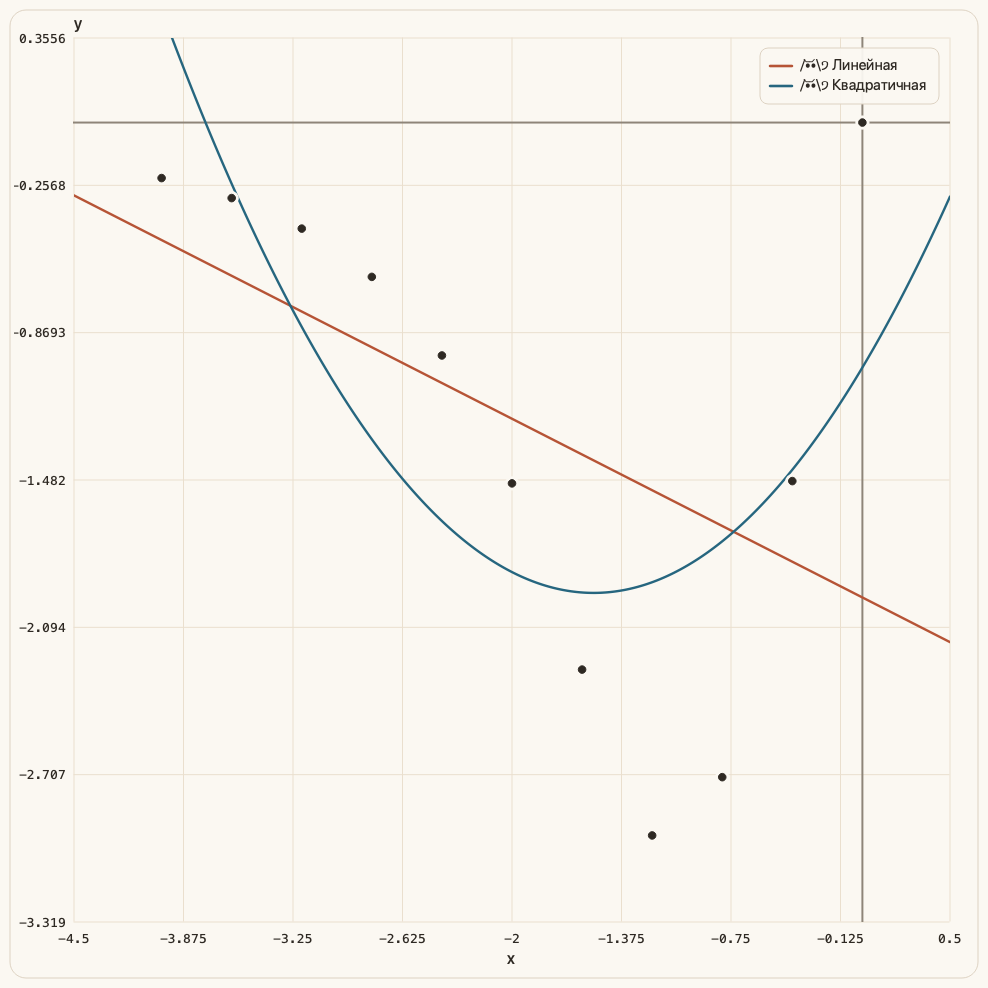
\includegraphics[width=0.85\textwidth]{report_assets/plot_variant4.png}
    \caption{Линейное и квадратичное приближения, построенные программой}
\end{figure}

\section*{Блок-схемы реализованных алгоритмов}
Блок-схемы построены по коду программы.

\begin{figure}[H]
    \centering
    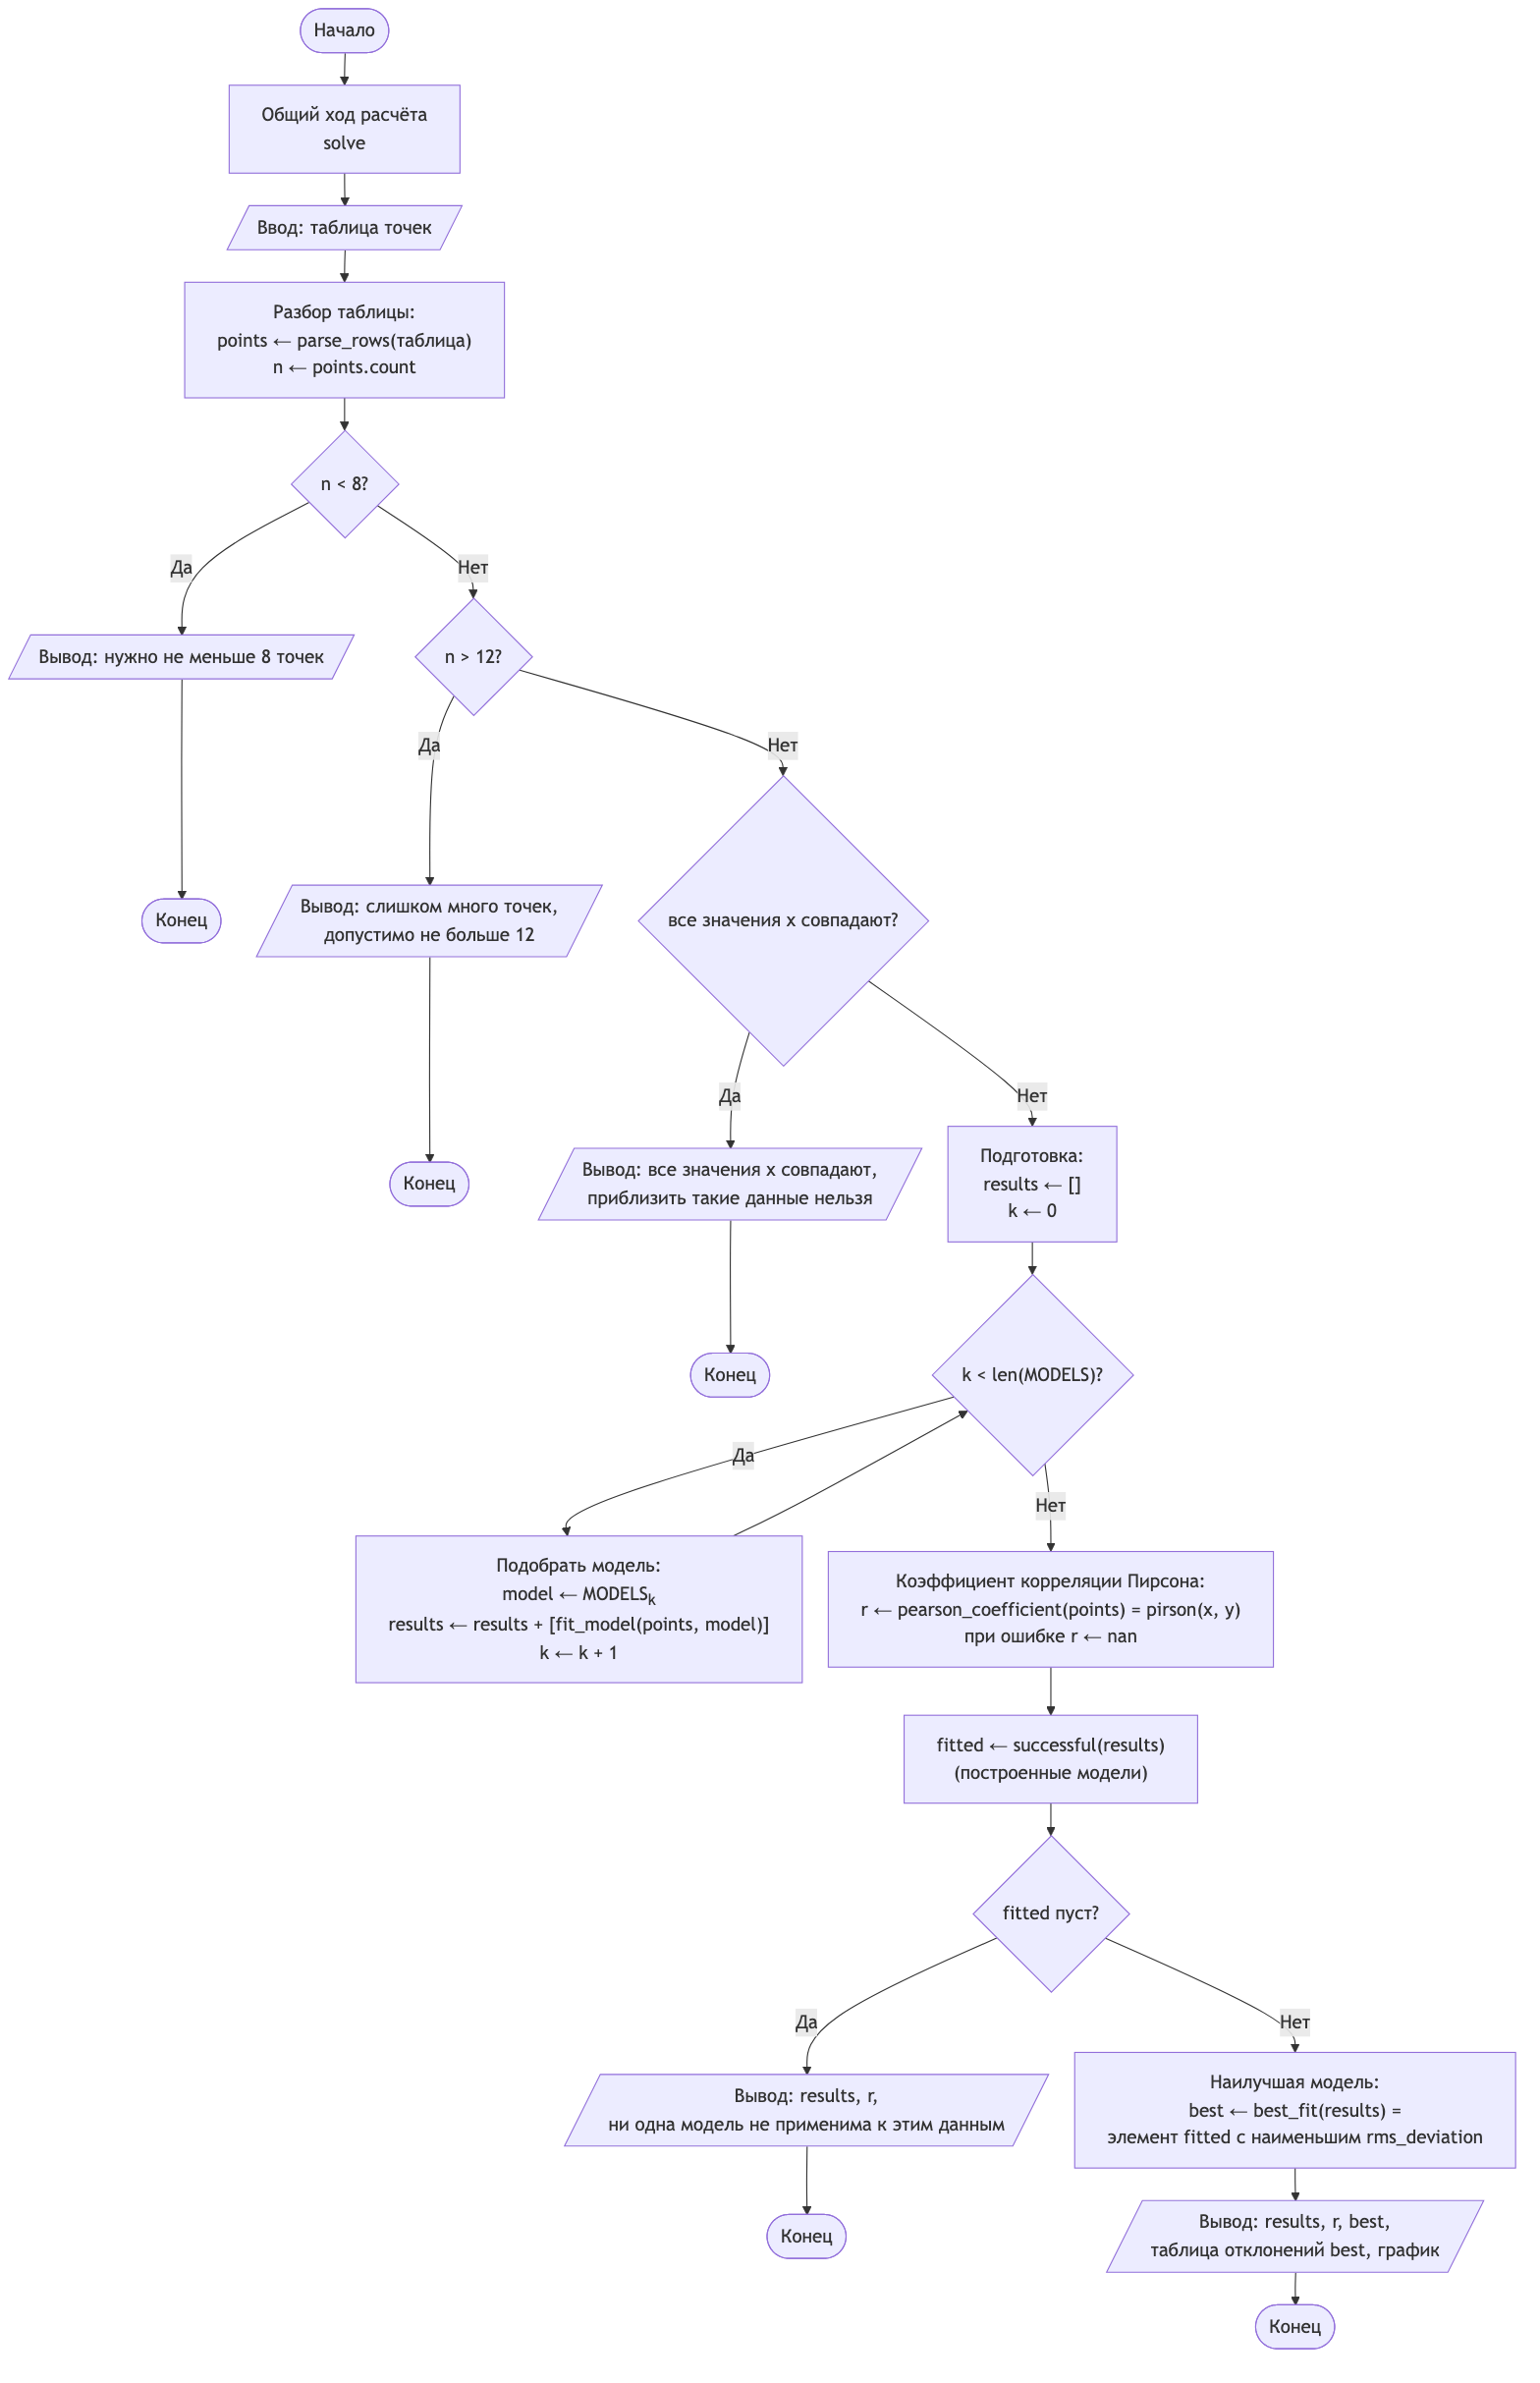
\includegraphics[width=\textwidth,height=0.82\textheight,keepaspectratio]{report_assets/solve.png}
    \caption{Блок-схема общего хода расчёта (функция \texttt{solve})}
\end{figure}

\begin{figure}[H]
    \centering
    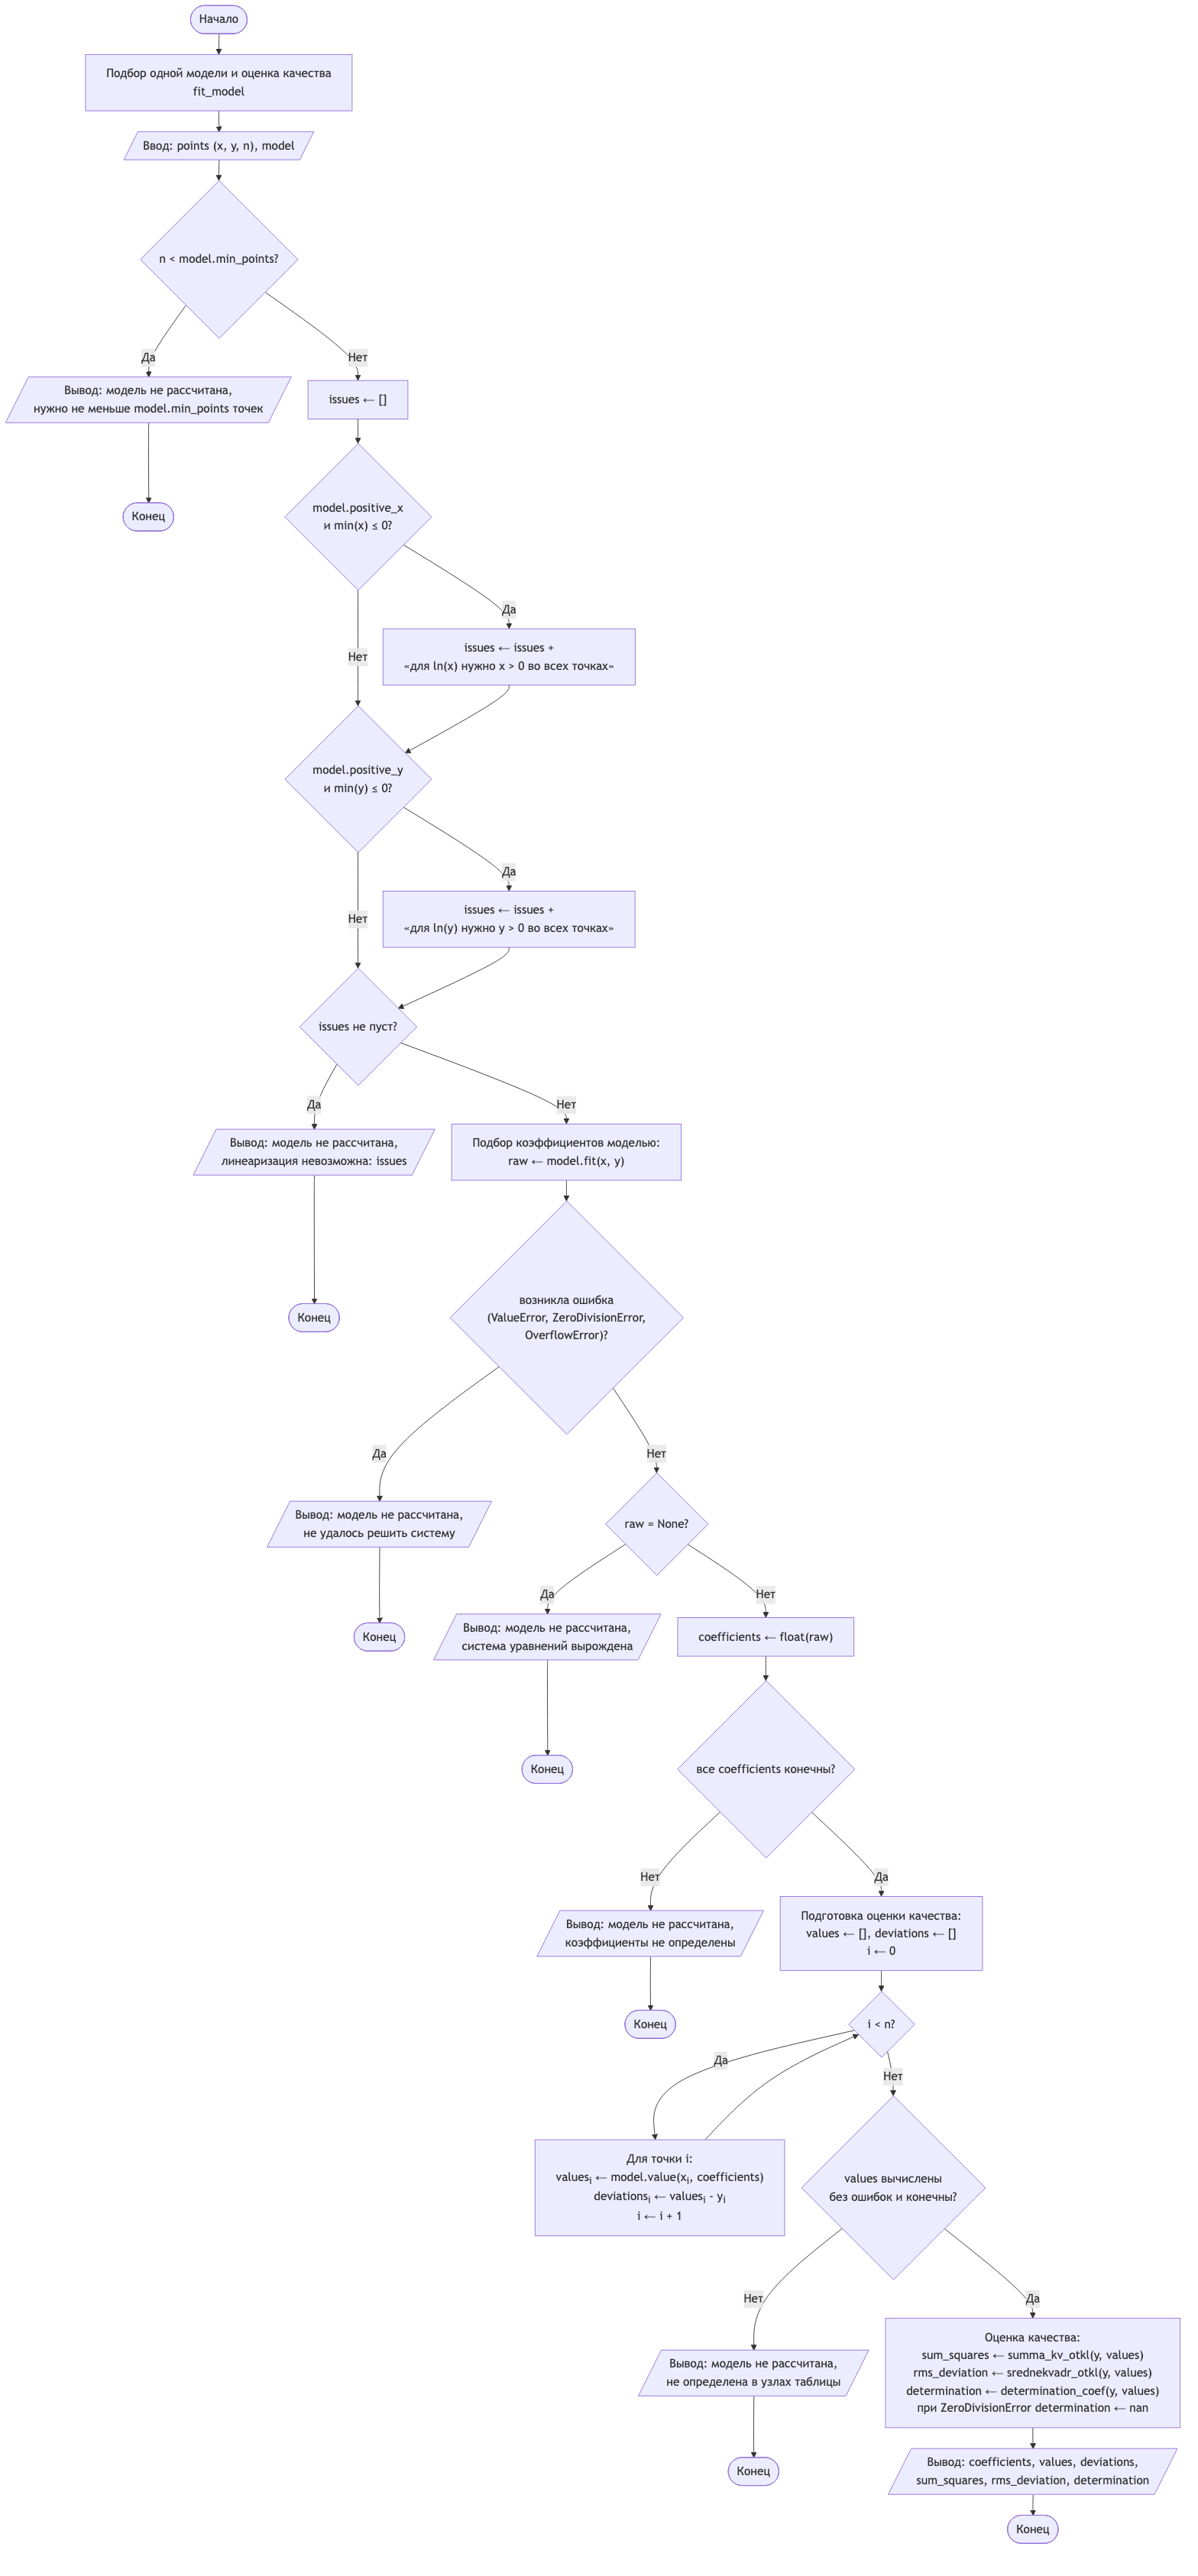
\includegraphics[width=\textwidth,height=0.82\textheight,keepaspectratio]{report_assets/fit_model.png}
    \caption{Блок-схема подбора одной модели и оценки качества (функция \texttt{fit\_model})}
\end{figure}

\begin{figure}[H]
    \centering
    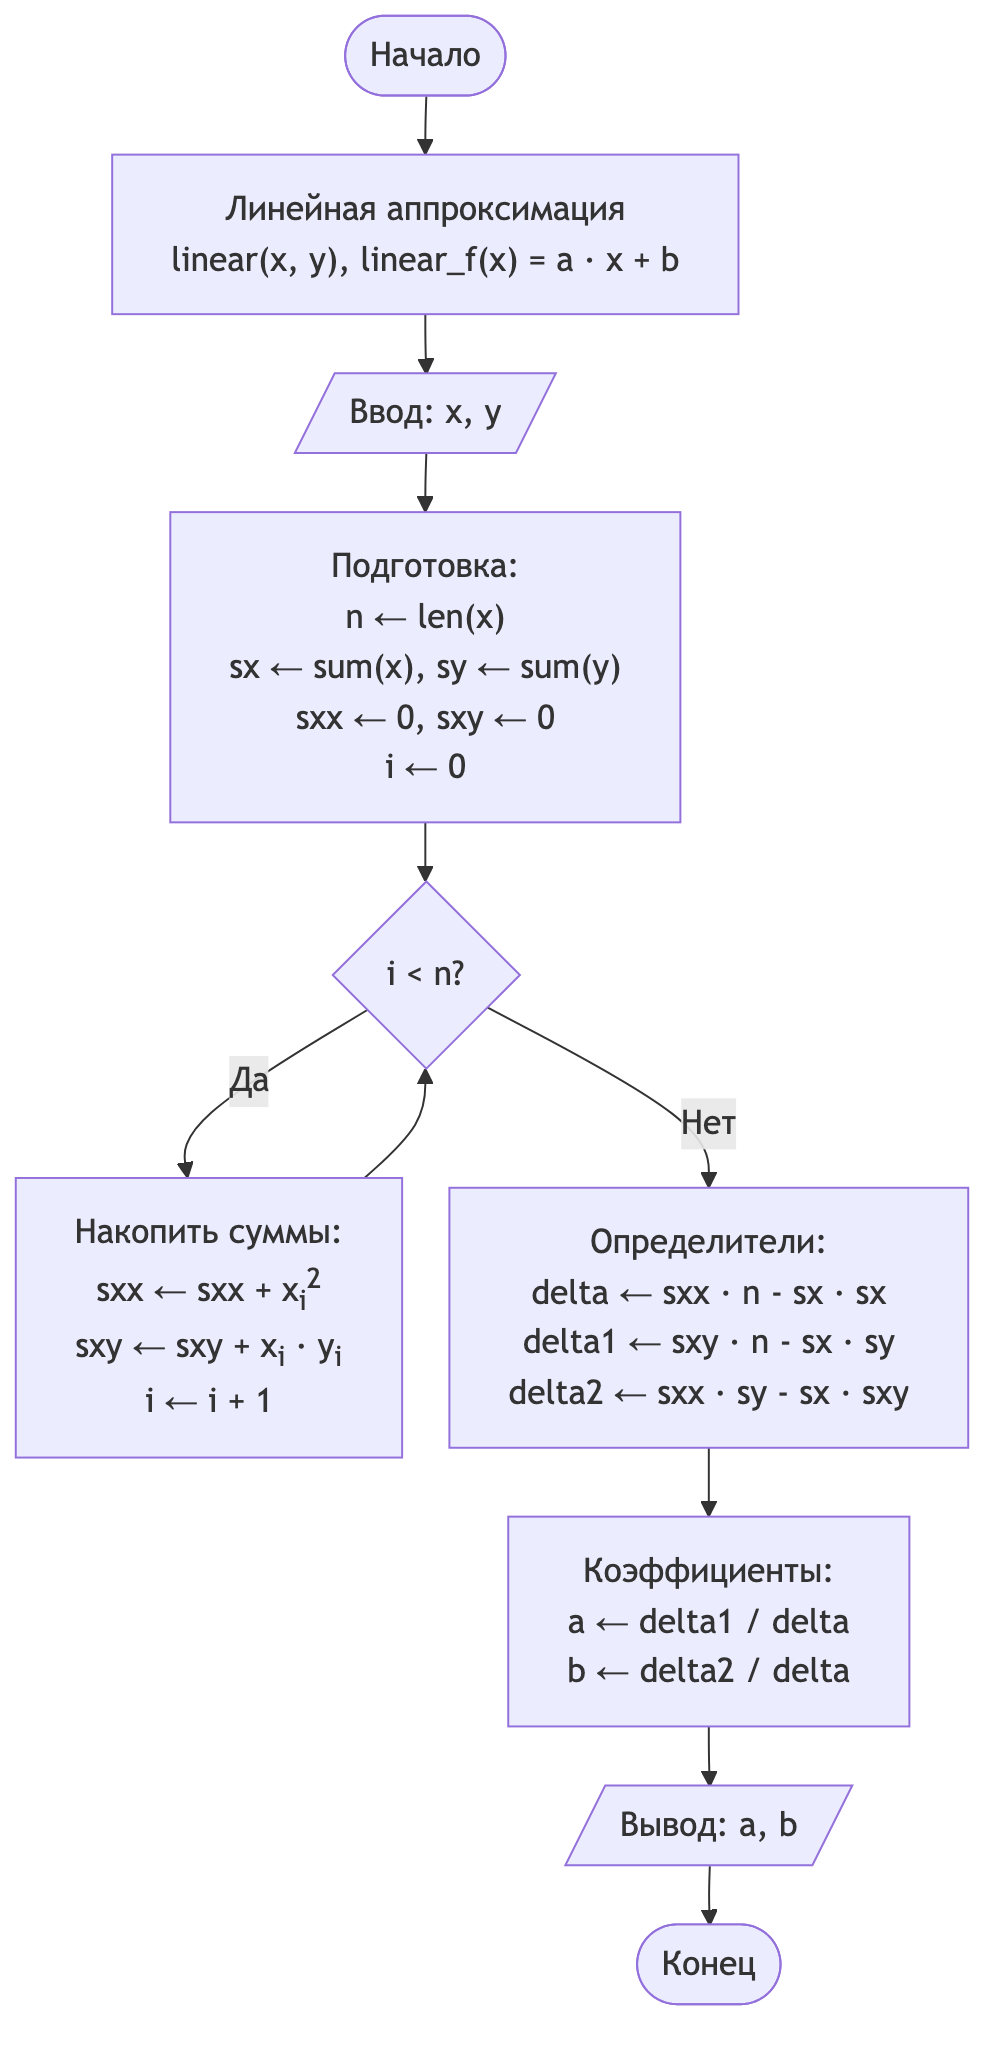
\includegraphics[width=\textwidth,height=0.82\textheight,keepaspectratio]{report_assets/linear.png}
    \caption{Блок-схема линейной аппроксимации (функция \texttt{linear})}
\end{figure}

\begin{figure}[H]
    \centering
    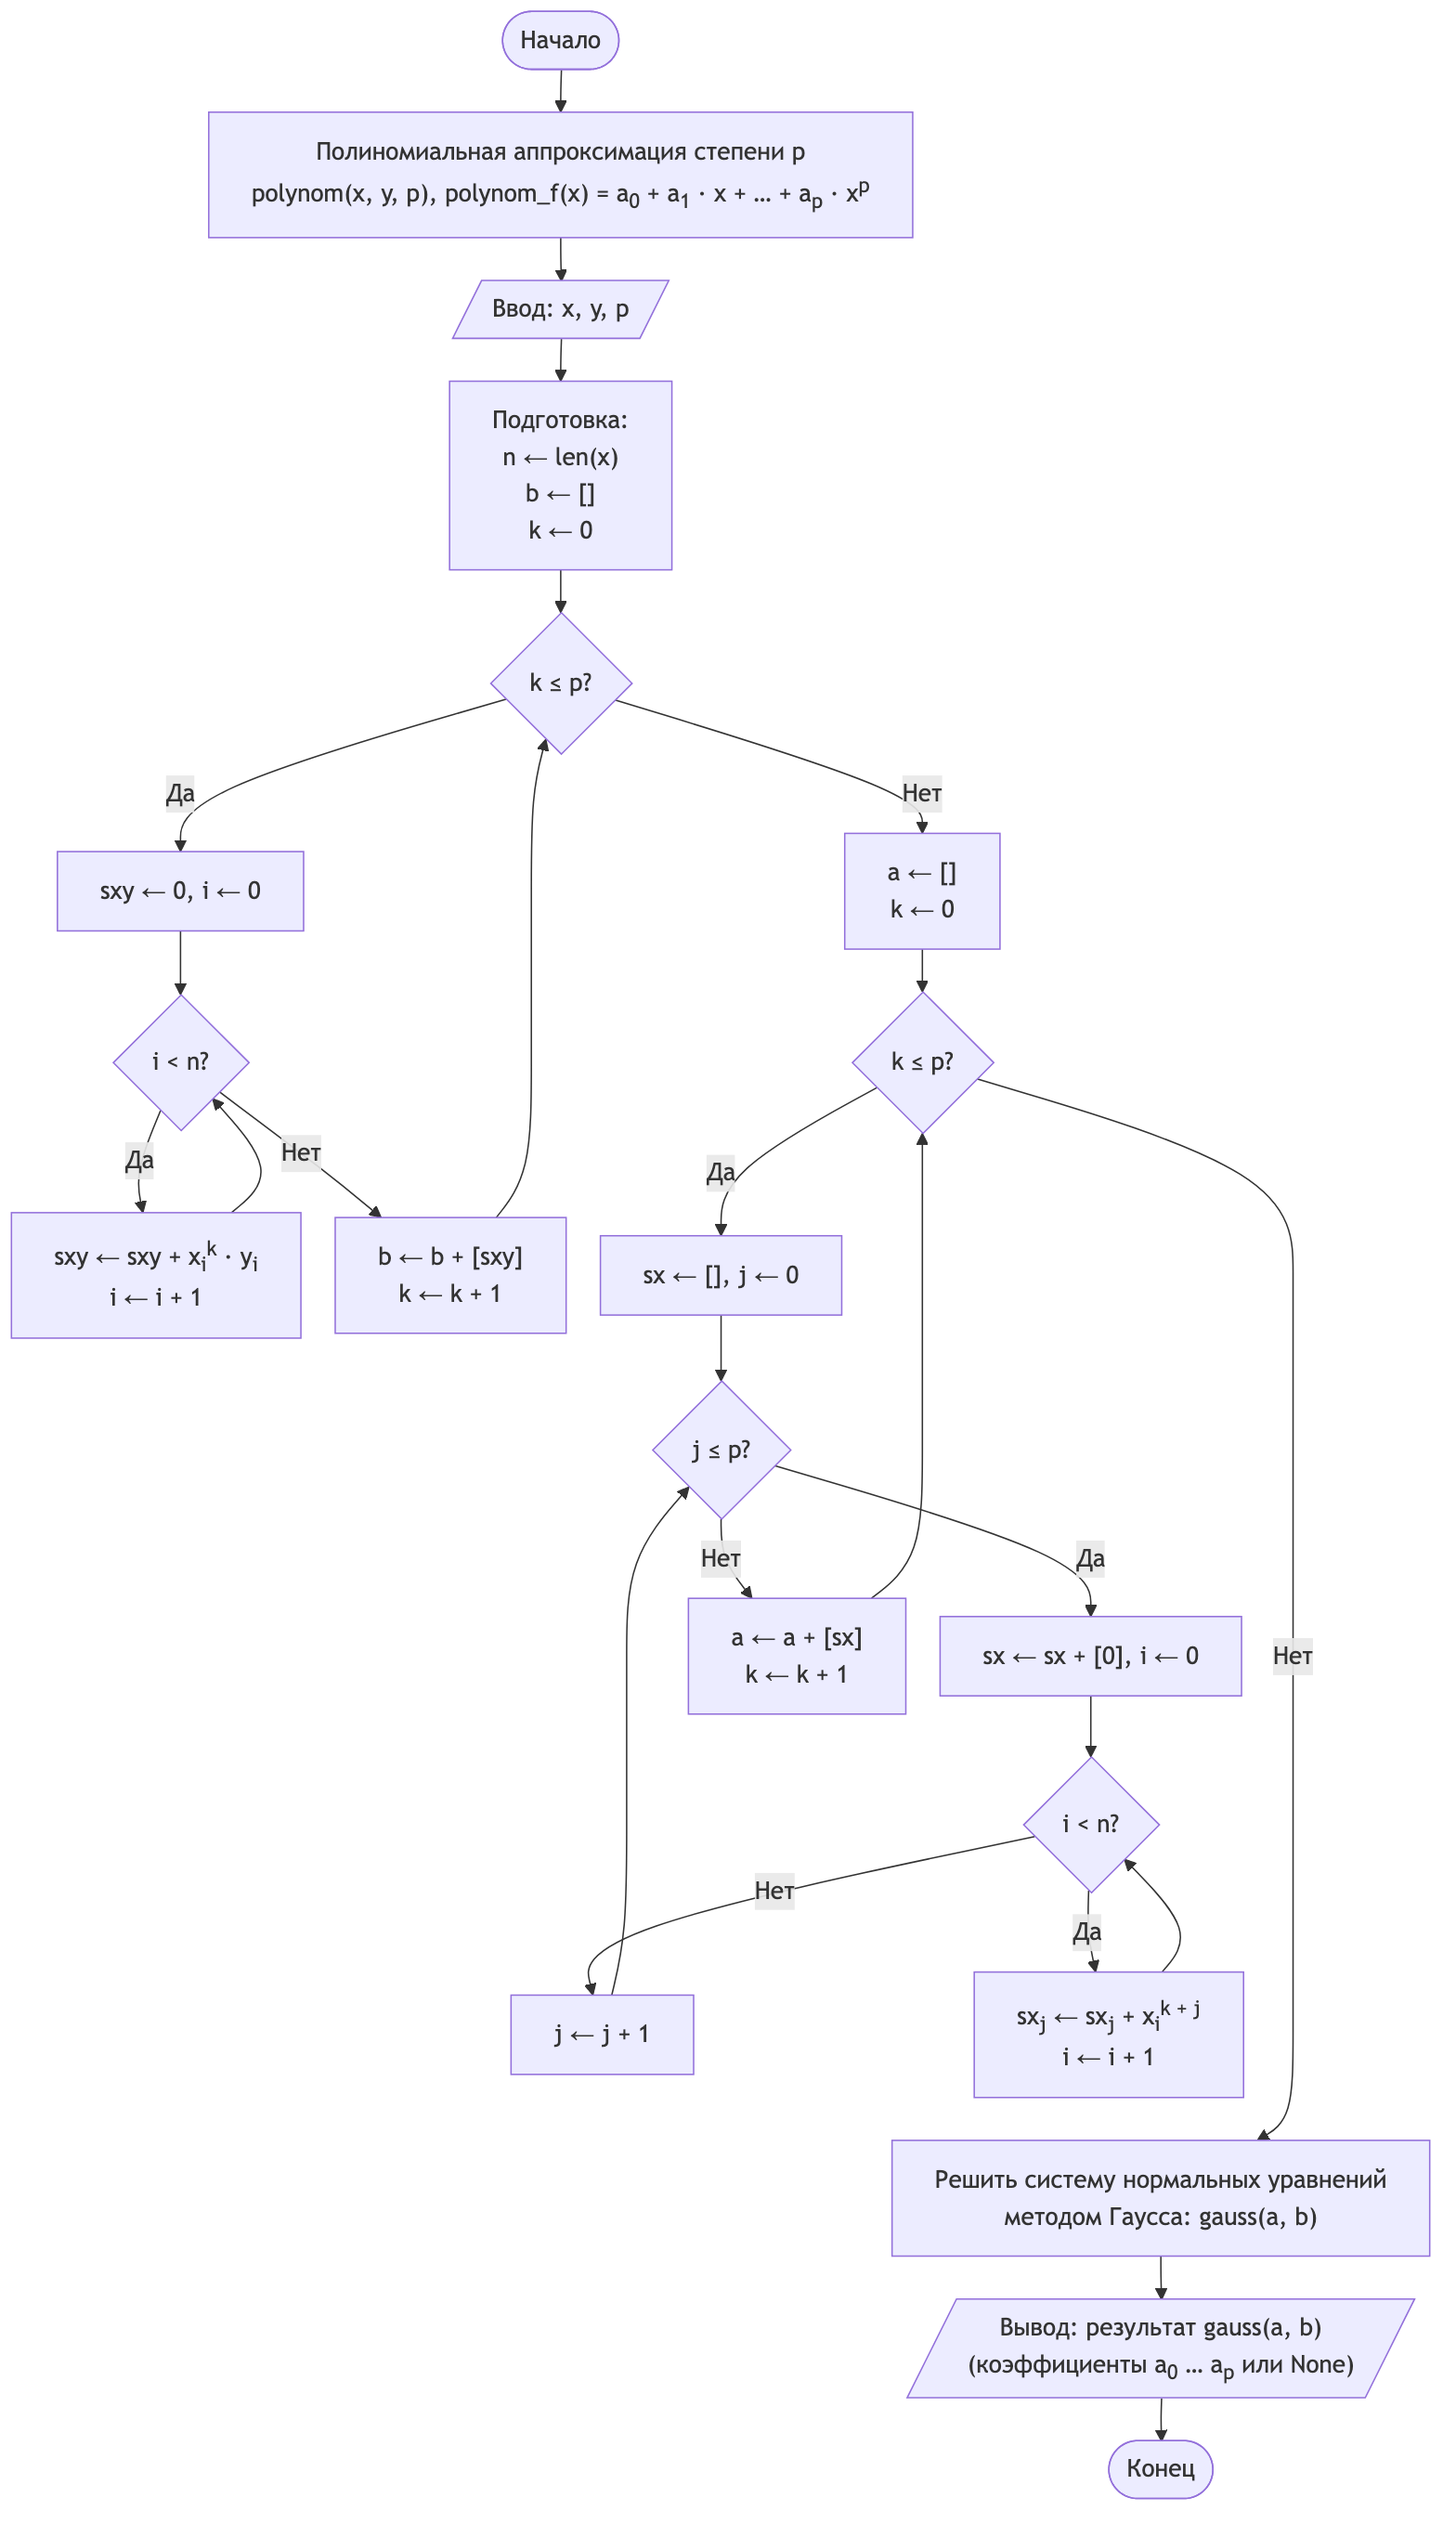
\includegraphics[width=\textwidth,height=0.82\textheight,keepaspectratio]{report_assets/polynom.png}
    \caption{Блок-схема полиномиальной аппроксимации (функция \texttt{polynom})}
\end{figure}

\begin{figure}[H]
    \centering
    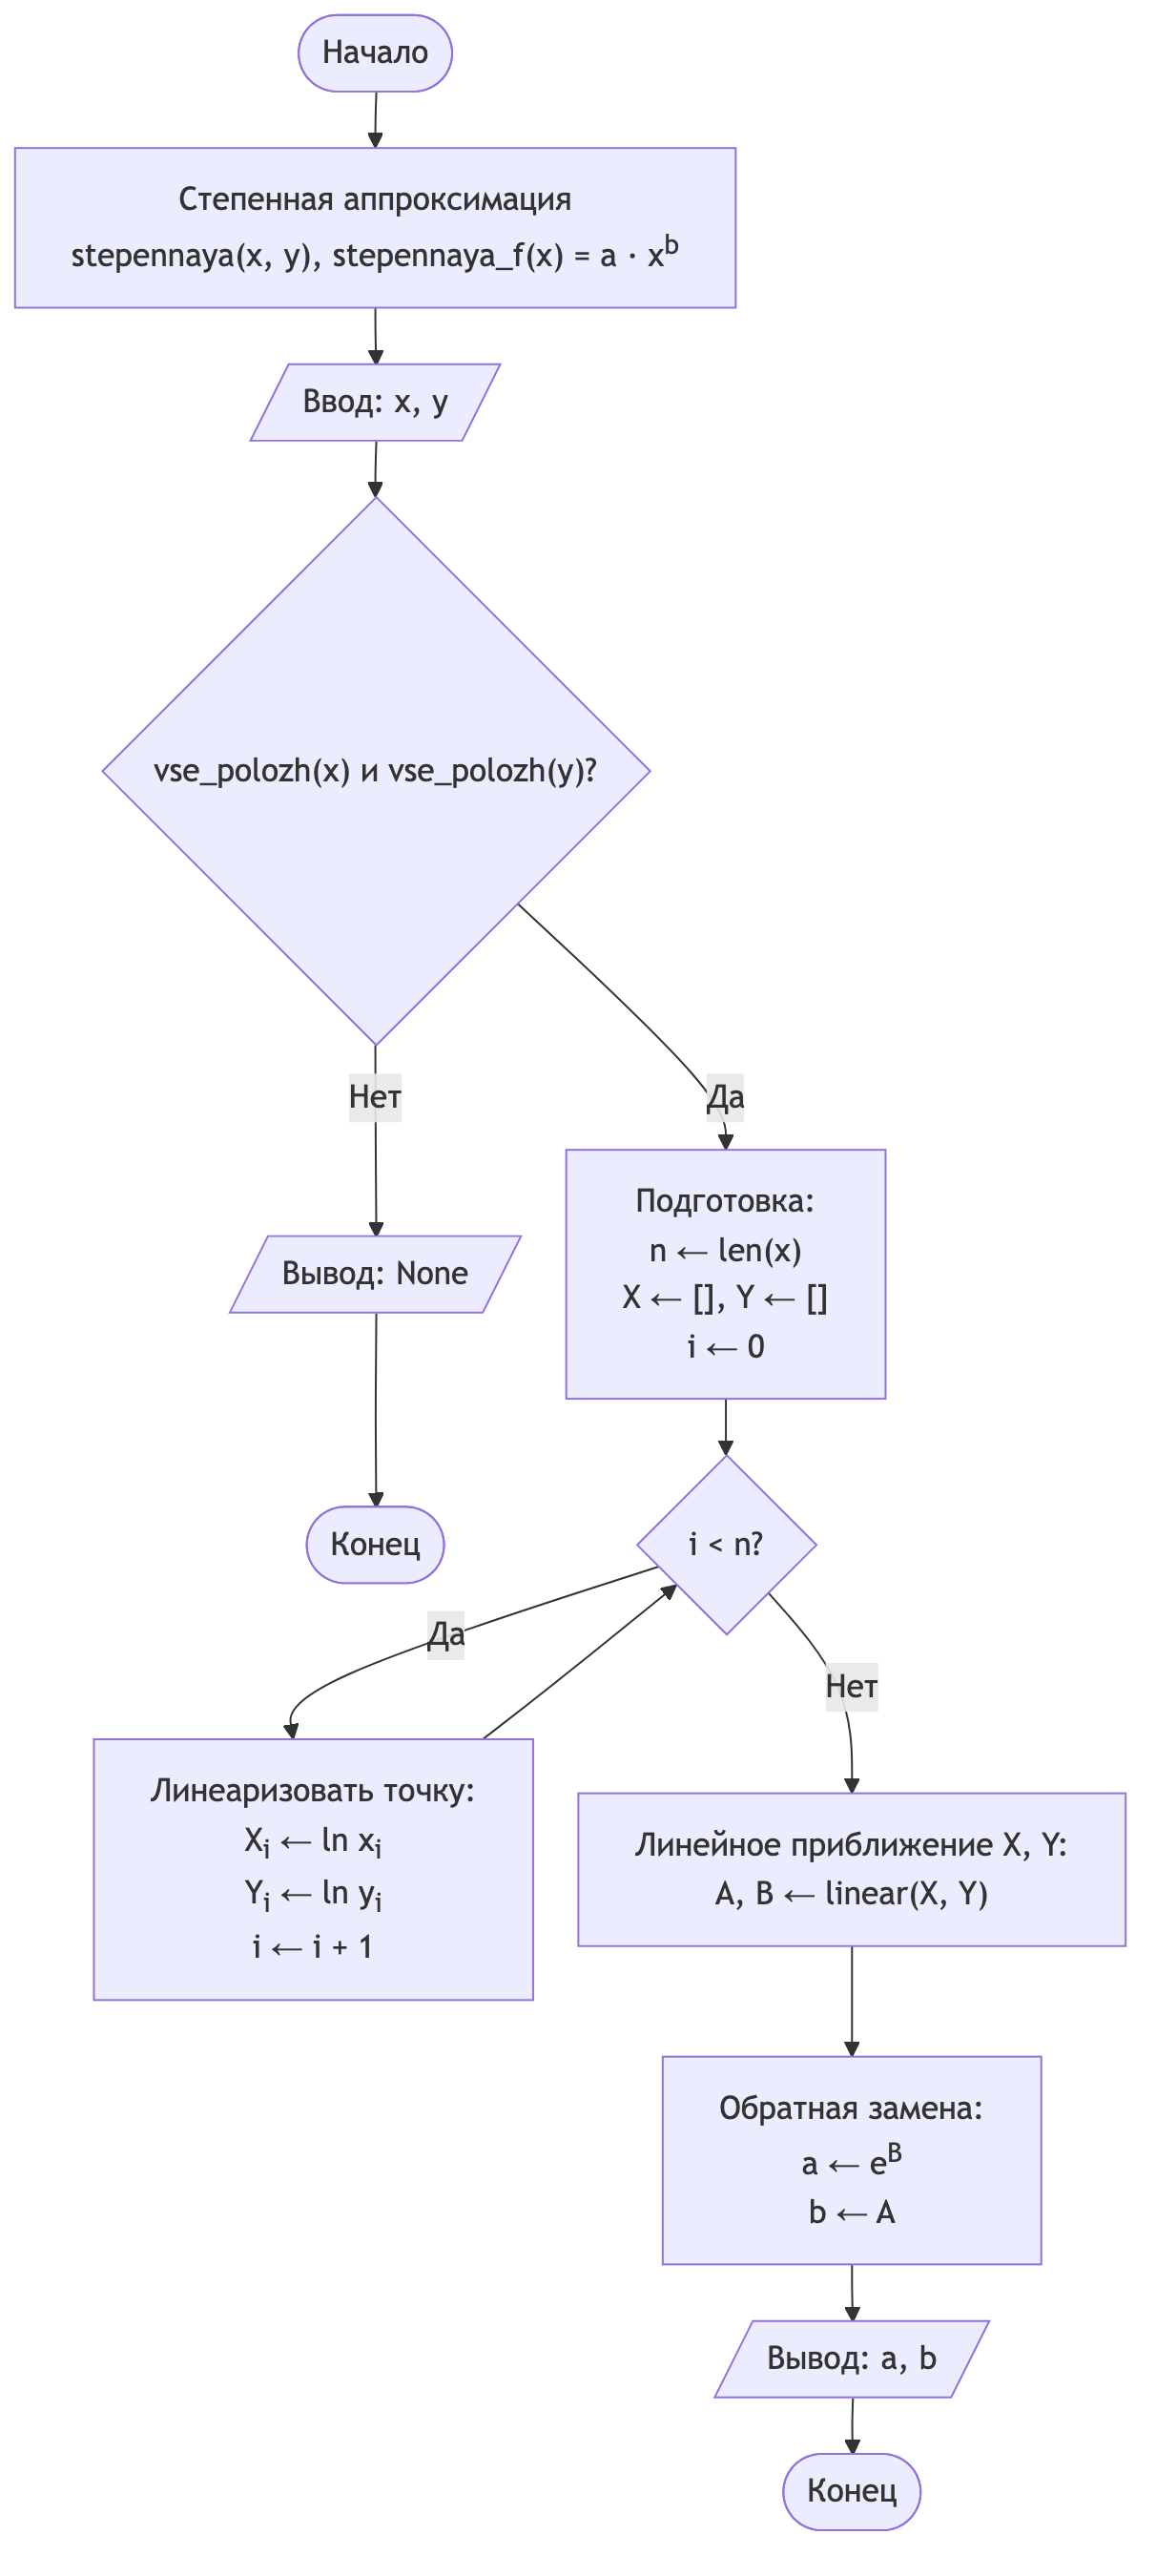
\includegraphics[width=\textwidth,height=0.82\textheight,keepaspectratio]{report_assets/stepennaya.png}
    \caption{Блок-схема степенной аппроксимации (функция \texttt{stepennaya})}
\end{figure}

\begin{figure}[H]
    \centering
    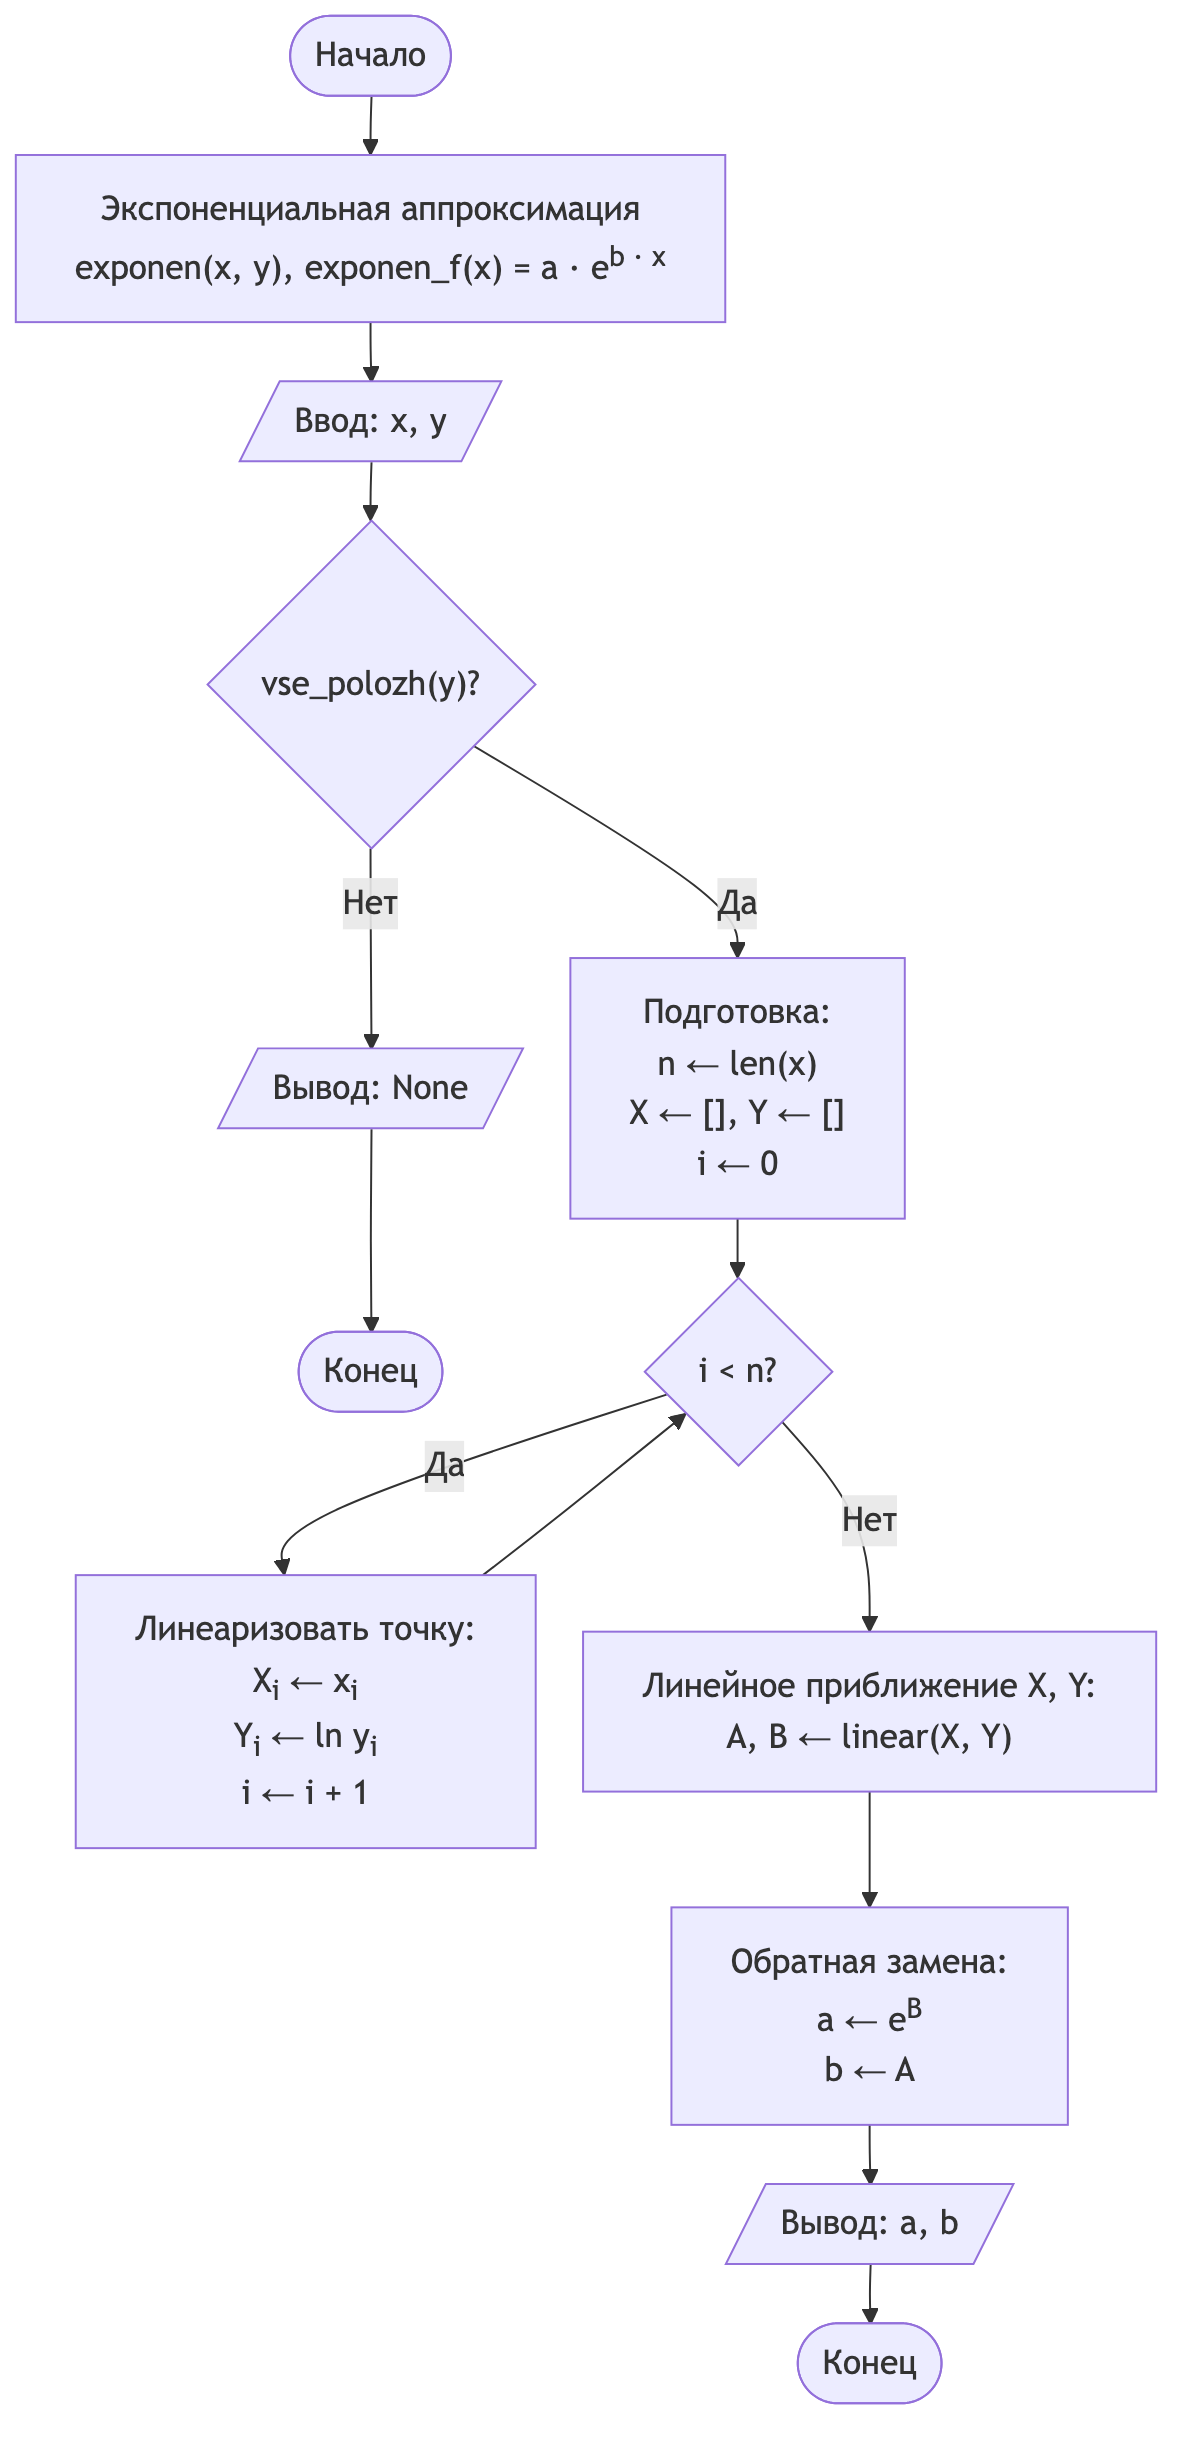
\includegraphics[width=\textwidth,height=0.82\textheight,keepaspectratio]{report_assets/exponen.png}
    \caption{Блок-схема экспоненциальной аппроксимации (функция \texttt{exponen})}
\end{figure}

\begin{figure}[H]
    \centering
    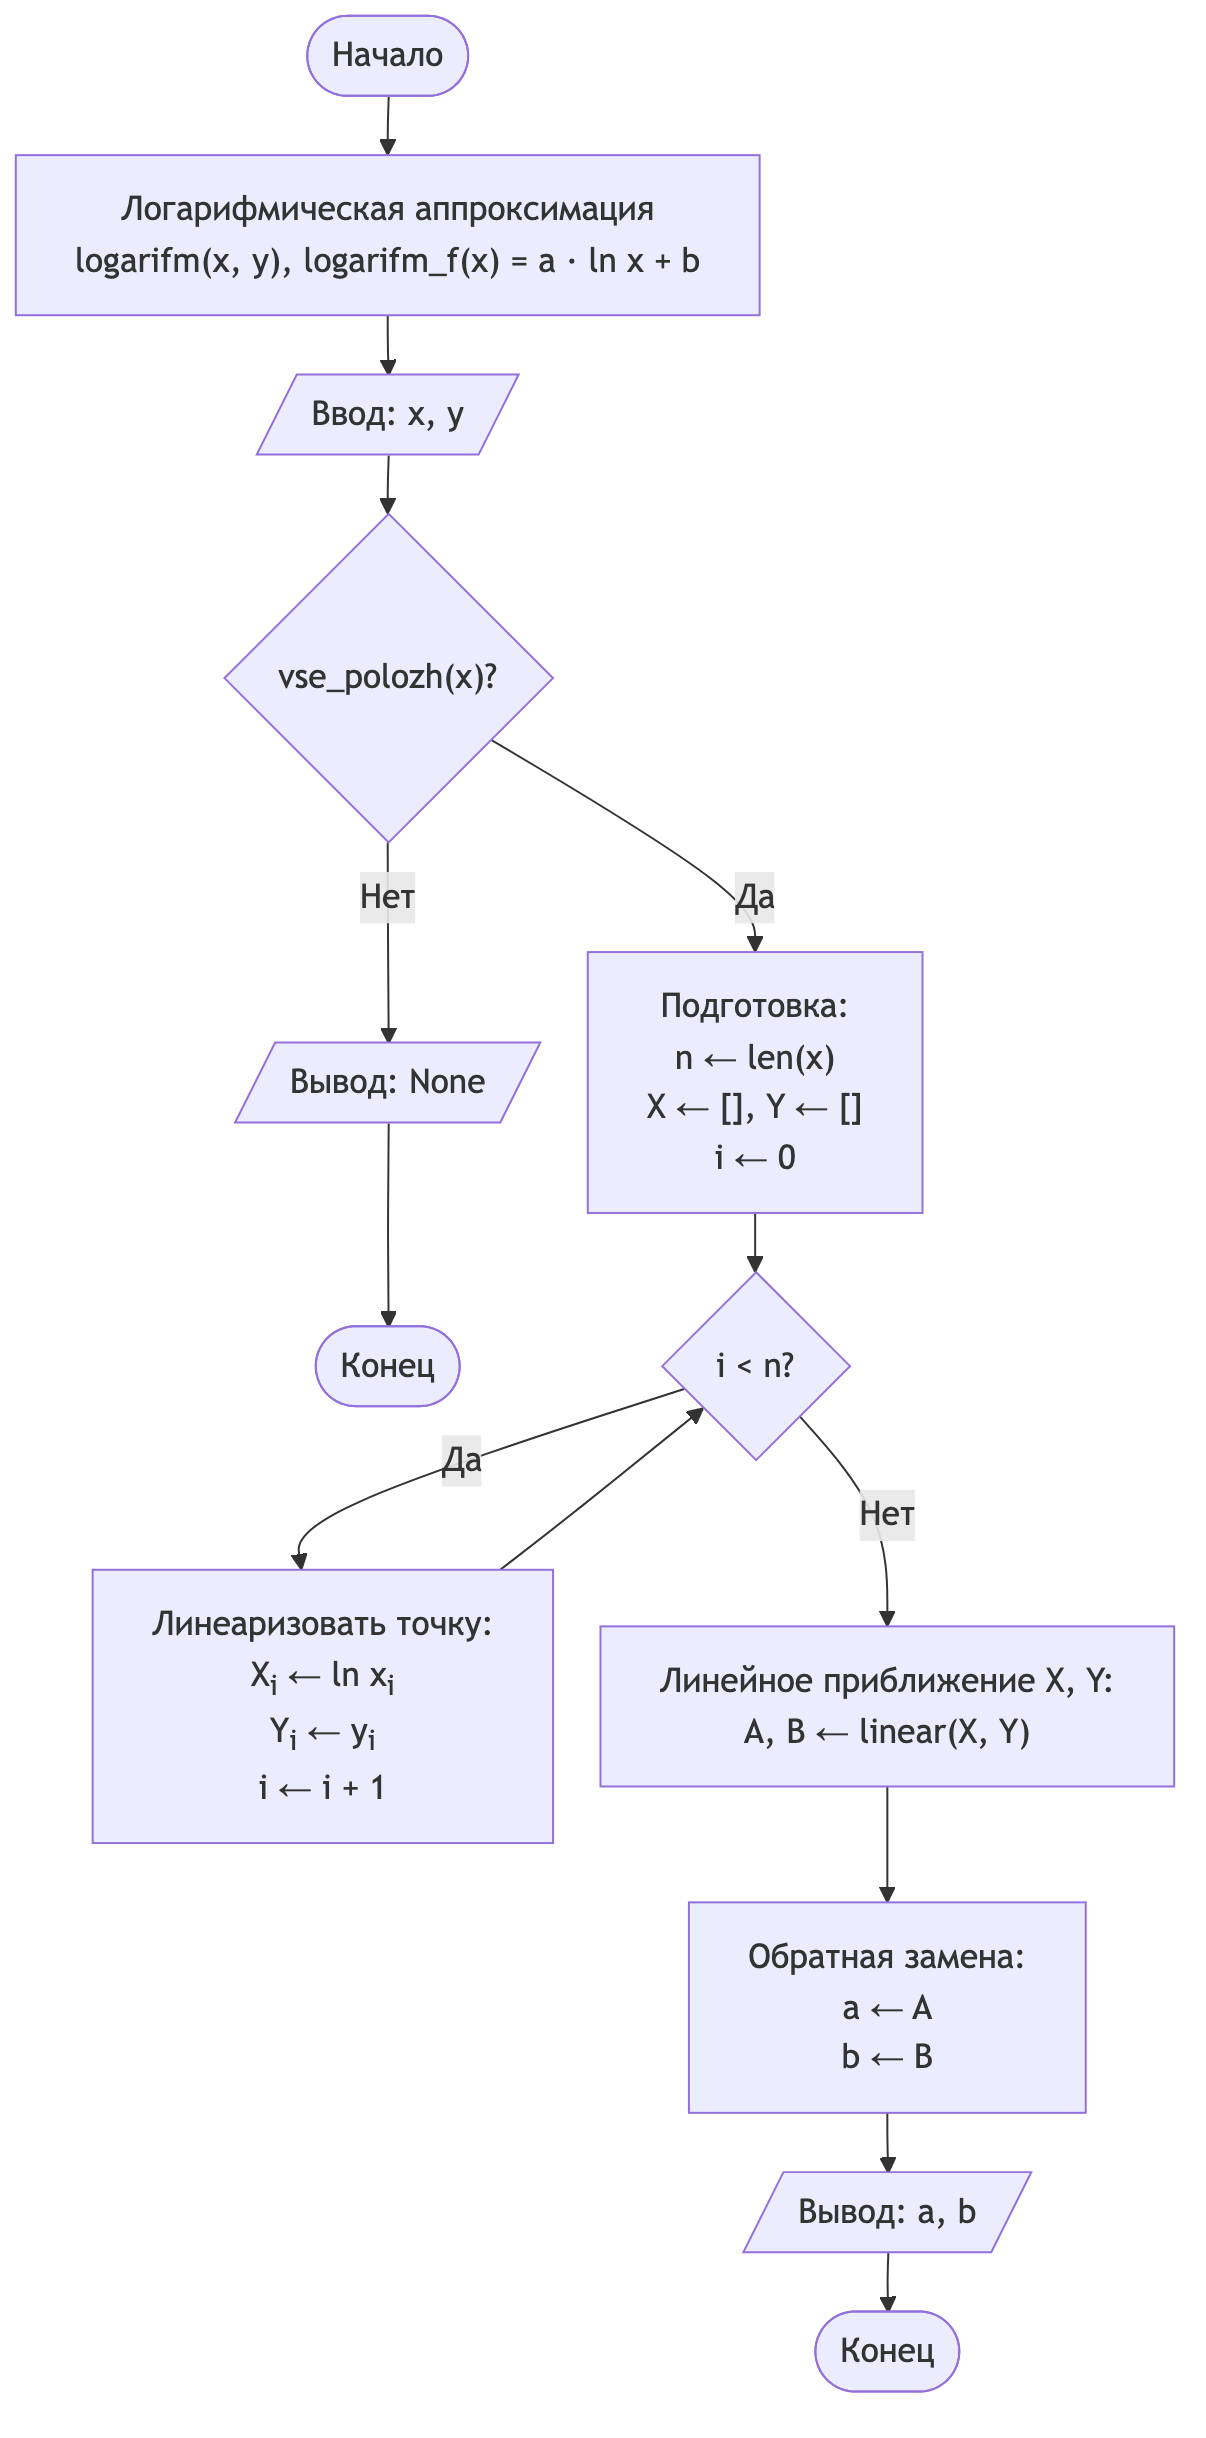
\includegraphics[width=\textwidth,height=0.82\textheight,keepaspectratio]{report_assets/logarifm.png}
    \caption{Блок-схема логарифмической аппроксимации (функция \texttt{logarifm})}
\end{figure}

\section*{Реализация численного метода}
Метод наименьших квадратов реализован в модуле \texttt{numerical.py}, проверки данных и оценка качества -- в \texttt{approximation.py}, интерфейс -- в \texttt{app.py} и \texttt{plotting.py}. Ниже приведён код функций \texttt{numerical.py}.

\subsection*{Линейная аппроксимация}
\begin{lstlisting}[language=Python,caption={Функция \texttt{linear}}]
def linear(x, y):
    n = len(x)
    sx = sum(x)
    sxx = 0
    for i in x:
        sxx += i**2

    sy = sum(y)
    sxy = 0
    for i in range(n):
        sxy += x[i] * y[i]

    delta = sxx * n - sx * sx
    delta1 = sxy * n - sx * sy
    delta2 = sxx * sy - sx * sxy

    a = delta1 / delta
    b = delta2 / delta

    return a, b
\end{lstlisting}

\subsection*{Решение системы линейных уравнений методом Гаусса}
\begin{lstlisting}[language=Python,caption={Функция \texttt{gauss}}]
def gauss(a, b):
    n = len(b)

    # расширенная матрица: к каждой строке A дописываем элемент b
    m = []
    for i in range(n):
        row = []
        for j in range(n):
            row.append(a[i][j])
        row.append(b[i])
        m.append(row)

    # прямой ход
    for k in range(n):
        # ищем главный элемент в k-м столбце
        glavnaya = k
        for i in range(k + 1, n):
            if abs(m[i][k]) > abs(m[glavnaya][k]):
                glavnaya = i

        if abs(m[glavnaya][k]) < 1e-12:
            return None  # матрица вырождена

        if glavnaya != k:
            tmp = m[k]
            m[k] = m[glavnaya]
            m[glavnaya] = tmp

        # обнуляем k-й столбец под диагональю
        for i in range(k + 1, n):
            c = m[i][k] / m[k][k]
            for j in range(k, n + 1):
                m[i][j] -= c * m[k][j]

    # обратный ход
    x = [0.0] * n
    for i in range(n - 1, -1, -1):
        summa = 0.0
        for j in range(i + 1, n):
            summa += m[i][j] * x[j]
        x[i] = (m[i][n] - summa) / m[i][i]

    return x
\end{lstlisting}

\subsection*{Полиномиальная аппроксимация}
\begin{lstlisting}[language=Python,caption={Функция \texttt{polynom}}]
def polynom(x, y, p):
    n = len(x)
    b = []
    for k in range(p+1):
        sxy = 0
        for i in range(n):
            sxy += x[i]**k * y[i]
        b.append(sxy)

    a = []
    for k in range(p+1):
        sx = []
        for j in range(p+1):
            sx.append(0)
            for i in range(n):
                sx[j] += x[i] ** (k+j)
        a.append(sx)

    return gauss(a, b) #ответ на аппроксимацию
\end{lstlisting}

\subsection*{Проверка положительности значений}
\begin{lstlisting}[language=Python,caption={Функция \texttt{vse\_polozh}}]
def vse_polozh(spisok):
    for i in spisok:
        if i <= 0:
            return False
    return True
\end{lstlisting}

\subsection*{Степенная аппроксимация}
\begin{lstlisting}[language=Python,caption={Функция \texttt{stepennaya}}]
def stepennaya(x, y):
    # ln x и ln y определены только при x > 0 и y > 0
    if not vse_polozh(x) or not vse_polozh(y):
        return None

    n = len(x)
    X = []
    Y = []
    for i in range(n):
        X.append(math.log(x[i]))
        Y.append(math.log(y[i]))
    A, B = linear(X, Y)
    a = math.exp(B)
    b = A
    return a, b
\end{lstlisting}

\subsection*{Экспоненциальная аппроксимация}
\begin{lstlisting}[language=Python,caption={Функция \texttt{exponen}}]
def exponen(x, y):
    # логарифмируем только y, поэтому нужно y > 0
    if not vse_polozh(y):
        return None

    n = len(x)
    X = []
    Y = []
    for i in range(n):
        X.append(x[i])
        Y.append(math.log(y[i]))
    A, B = linear(X, Y)
    a = math.exp(B)
    b = A
    return a, b
\end{lstlisting}

\subsection*{Логарифмическая аппроксимация}
\begin{lstlisting}[language=Python,caption={Функция \texttt{logarifm}}]
def logarifm(x, y):
    # заменяем только аргумент, поэтому нужно x > 0
    if not vse_polozh(x):
        return None

    n = len(x)
    X = []
    Y = []
    for i in range(n):
        X.append(math.log(x[i]))
        Y.append(y[i])
    A, B = linear(X, Y)
    a = A
    b = B
    return a, b
\end{lstlisting}

\subsection*{Мера отклонения}
\begin{lstlisting}[language=Python,caption={Функция \texttt{summa\_kv\_otkl}}]
def summa_kv_otkl(y_old, y_new):
    s = 0
    n = len(y_old)
    for i in range(n):
        s += (y_new[i] - y_old[i]) ** 2
    return s
\end{lstlisting}

\subsection*{Среднеквадратичное отклонение}
\begin{lstlisting}[language=Python,caption={Функция \texttt{srednekvadr\_otkl}}]
def srednekvadr_otkl(y_old, y_new):
    n = len(y_old)
    b = math.sqrt(summa_kv_otkl(y_old, y_new) / n)
    return b
\end{lstlisting}

\subsection*{Коэффициент детерминации}
\begin{lstlisting}[language=Python,caption={Функция \texttt{determination\_coef}}]
def determination_coef(y_old, y_new):
    n = len(y_old)
    niz = 0
    sr_sum_y_new = sum(y_new) / n
    for i in range(n):
        niz += (y_old[i] - sr_sum_y_new) ** 2
    r2 = 1 - summa_kv_otkl(y_old, y_new) / niz
    return r2
\end{lstlisting}

\subsection*{Коэффициент корреляции Пирсона}
\begin{lstlisting}[language=Python,caption={Функция \texttt{pirson}}]
def pirson(x, y):
    n = len(x)
    x_cp = sum(x) / n
    y_cp = sum(y) / n
    verx = 0
    niz_x = 0
    niz_y = 0
    for i in range(n):
        verx += (x[i] - x_cp) * (y[i] - y_cp)
        niz_x += ((x[i] - x_cp)**2)
        niz_y += ((y[i] - y_cp)**2)
    niz = math.sqrt(niz_x * niz_y)
    r = verx/niz
    return r


if __name__ == "__main__":
    x = [-1, 2, -3, 0, -3.0000009845849594848999999]
    y = [-7, -15, 28, 1000, -9]
    a = polynom(x, y, 3)
    n = len(x)
    y_new = []
    for i in range(n):
        y_new.append(polynom_f(x[i], a))
    print(determination_coef(y, y_new), srednekvadr_otkl(y, y_new))
    print(a)
\end{lstlisting}

\section*{Пример работы}
Точки вводятся в таблицу вручную, кликом по графику или из файла; десятичный разделитель -- точка или запятая. Расчёт выполняется по всем шести моделям.

\subsection*{Набор 1: функция варианта 4}
Для табулированной функции варианта 4 на отрезке $[-4;0]$ по 11 точкам программа получает:
\begin{quote}
    Построено моделей: 3 из 6. Линейная: $\delta=0{,}87489$; квадратичная: $\delta=0{,}66976$; кубическая: $\delta=0{,}23991$. Наилучшая модель -- кубическая.
\end{quote}
Степенная, экспоненциальная и логарифмическая модели не построены: на этом интервале $x\le 0$ и $y\le 0$, поэтому необходимые для линеаризации логарифмы не определены. Программа выводит для каждой из них причину отказа.

\begin{figure}[H]
    \centering
    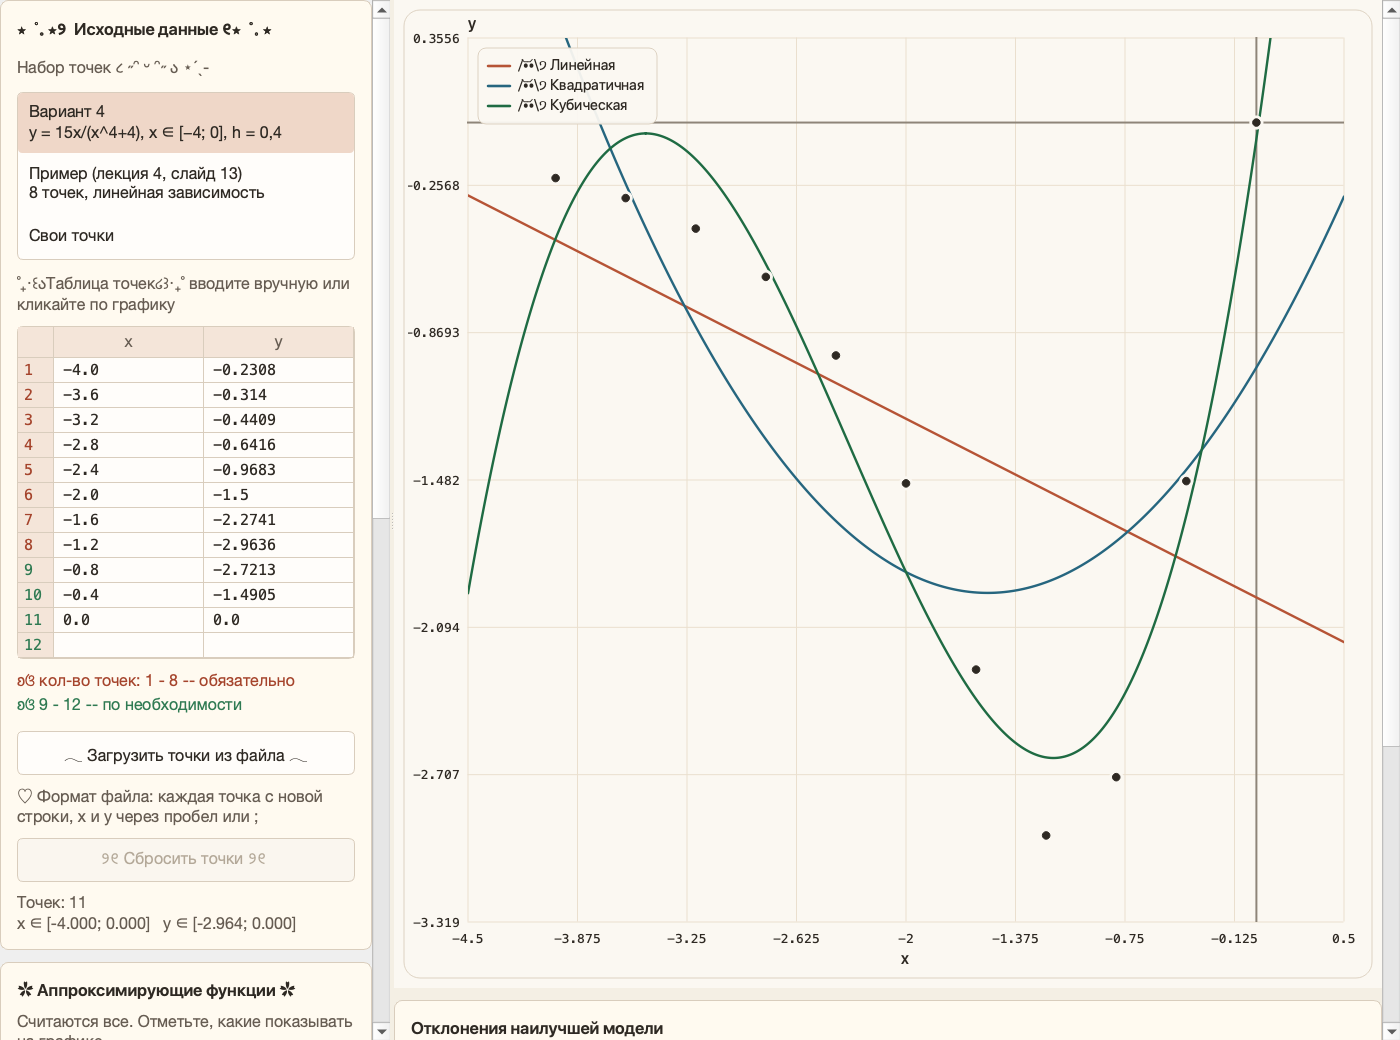
\includegraphics[width=\textwidth]{report_assets/screenshot_variant4.png}
    \caption{Пример работы программы для функции варианта 4}
\end{figure}

\subsection*{Набор 2: данные с положительными $x$ и $y$}
Для таблицы из 8 точек с положительными значениями строятся все шесть моделей:
\begin{quote}
    Построено моделей: 6 из 6. Коэффициент корреляции Пирсона $r=0{,}9954$. Линейная: $a=1{,}454330$, $b=5{,}291060$, $S=1{,}34585$, $\delta=0{,}41016$, $R^2=0{,}9909$ -- высокая точность аппроксимации. Наилучшая модель -- кубическая, $\delta=0{,}35348$.
\end{quote}

\begin{figure}[H]
    \centering
    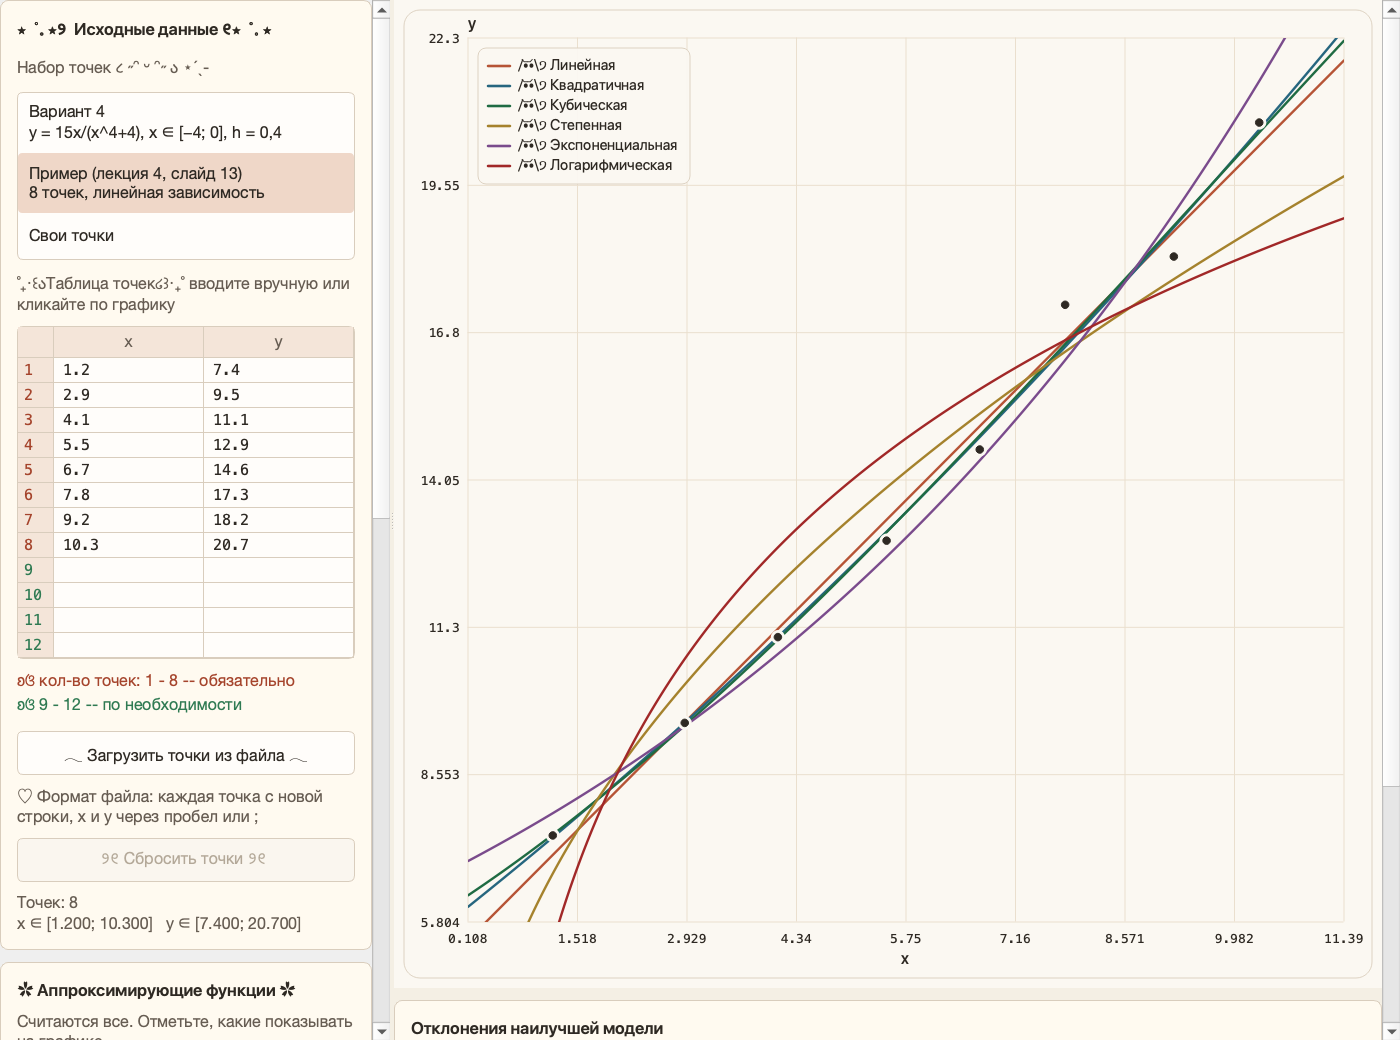
\includegraphics[width=\textwidth]{report_assets/screenshot_lecture.png}
    \caption{Пример работы программы при построении всех шести моделей}
\end{figure}

\subsection*{Набор 3: некорректные данные}
Если в таблице меньше 8 точек, расчет не выполняется:
\begin{quote}
    <<Нужно не меньше 8 точек, введено 5.>>
\end{quote}
Если точек больше 12, выводится сообщение:
\begin{quote}
    <<Слишком много точек: 13, допустимо не больше 12.>>
\end{quote}
Если все значения $x$ совпадают или в строке заполнено только одно из двух полей, программа также сообщает об ошибке, например:
\begin{quote}
    <<Все значения x совпадают, приблизить такие данные нельзя.>>
\end{quote}

\begin{figure}[H]
    \centering
    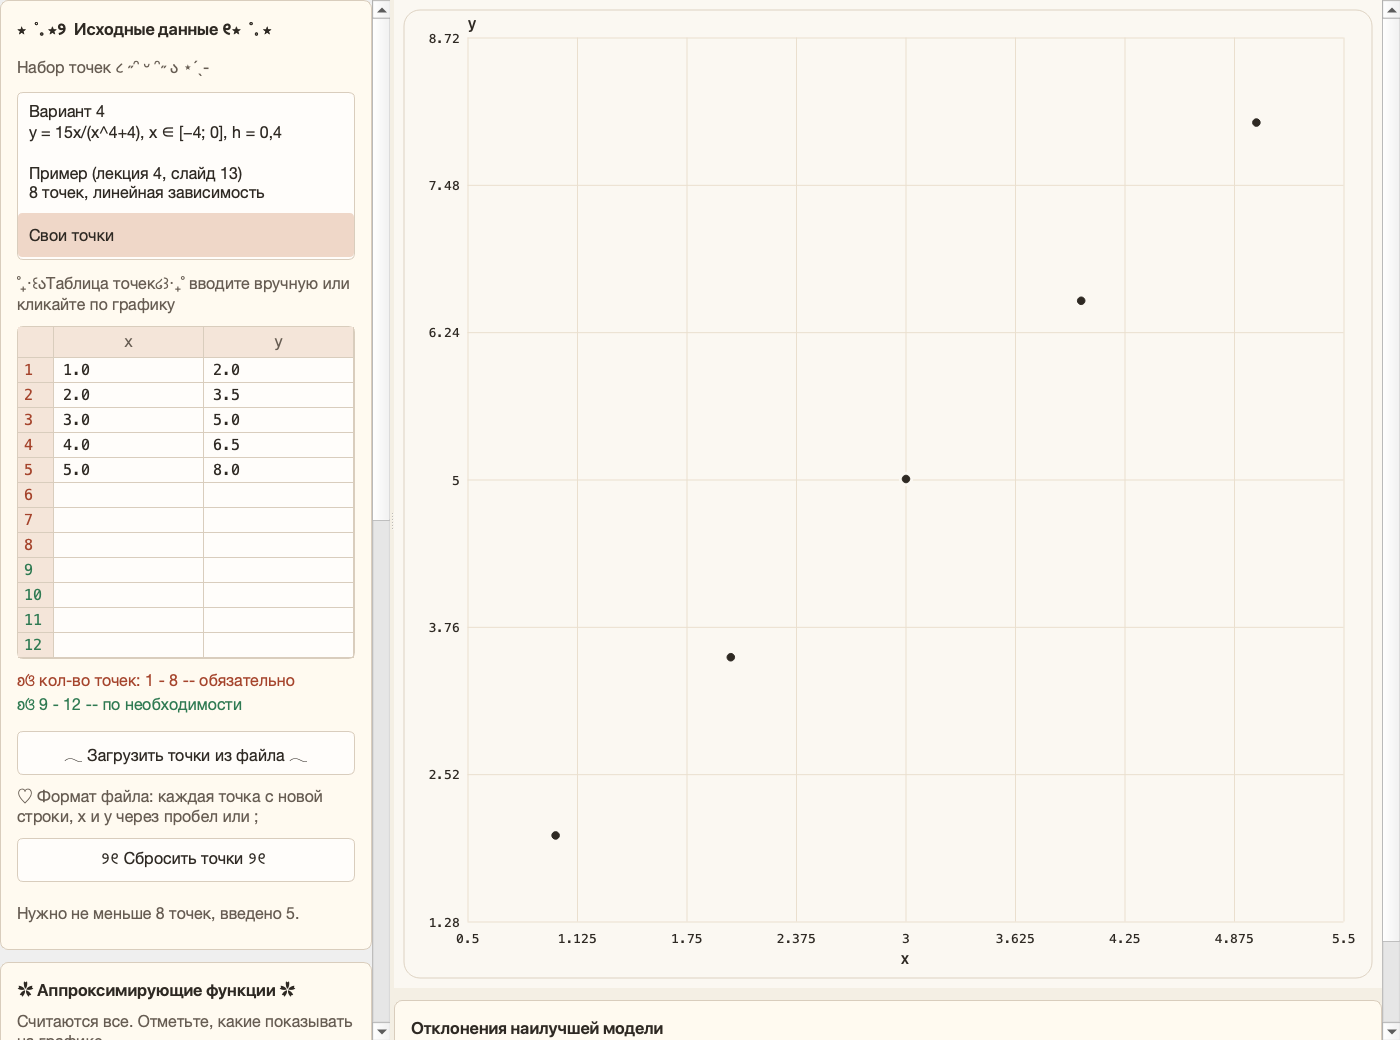
\includegraphics[width=\textwidth]{report_assets/screenshot_invalid.png}
    \caption{Реакция программы на недостаточное число точек}
\end{figure}

\section*{Ссылка на GitHub}
\url{https://github.com/juliakrasnoshtanova/itmo_compmath_lab4}

\section*{Вывод}
Реализована программа аппроксимации табличной функции методом наименьших квадратов для шести моделей: линейной, полиномиальных 2-й и 3-й степени, степенной, экспоненциальной и логарифмической. Для каждой модели программа выводит коэффициенты, меру отклонения, среднеквадратичное отклонение, коэффициент детерминации с оценкой точности и массивы $x_i$, $y_i$, $\varphi(x_i)$, $\varepsilon_i$; для линейной зависимости -- коэффициент корреляции Пирсона. Для функции варианта 4 в вычислительной части лучшим из двух приближений оказалось квадратичное, а среди всех моделей программы -- полиномиальное 3-й степени.

\end{document}
